
\documentclass{beamer}	
\mode<presentation>
 
\usepackage{pdfpages}
\usepackage{fancyvrb}
\usepackage{chemarr}

\usepackage{amsmath}		%% mathematics typesetting
\usepackage{amssymb}
 
\usepackage{epigraph}   %% nice setting of quotations

\usepackage{tabularx} %% allows to use row colours in tables

\usepackage{ulem}

\usepackage{booktabs}

\usepackage{siunitx} %% tpyeset SI units

\usepackage{CJKutf8} %% typeset Chinese characters

\usepackage{pdfpages}%% include pdfs

\usepackage{graphicx}
\usepackage{animate} %% show animated gifs

\DeclareMathAlphabet{\mathcalligra}{T1}{calligra}{m}{n}


% Color and Theme. Can be changed. However, this one's quite nice.
\usetheme{Madrid}
\definecolor{theme}{rgb}{0.84,0,0.21}
\usecolortheme[named=theme]{structure}

%%  Title information
\title[M01.9 Repetitorium Physik]{M01.9 Repetitorium Physik \\ Teil 2}
\author[melanie.stefan@medicalschool-berlin.de]{}
\institute[]{Prof. Ervice Pouokam Kamgne, Prof. Melanie Stefan \\ melanie.stefan@medicalschool-berlin.de}
\date{SoSe 23}
 

% Table of contents to pop up at the beginning of each section
\AtBeginSection[]
{
  \begin{frame}<beamer>
    \frametitle{Outline}
    \tableofcontents[currentsection,currentsubsection]
  \end{frame}
}
 
\beamertemplatenavigationsymbolsempty

\begin{document}


{ \usebackgroundtemplate{
\includegraphics[width=1.2\paperwidth]{MSB_Titelseite.pdf}} 
\begin{frame}

 \maketitle 

$\,$\\[6cm] 
\end{frame}
}

\section{M01.1 Methodik, Grundbegriffe, Fehlerrechnung}

%% Rechnen allgemein

% % Basiseinheiten und häufige abgeleitete Einheiten des SI-Systems benennen
% %  Vektoren, Skalare, Exponentialfunktionen, Logarithmen, Trigonometrischen Funktionen, Integration und Differentialrechnung erklären
%     %  Dezimale Vielfache von Einheiten sprachlich und durch Zehnerpotenzen darstellen
%     % mit Funktionsgraphen arbeiten
% % erkennen, warum Physik in der Medizin wichtig ist
% %  rechnen ohne Angst


\begin{frame}{Rechnen}
    


\begin{columns}[c]
\begin{column}{6cm}

% frequently used einheiten
\begin{block}{SI Einheiten}
\begin{center}
    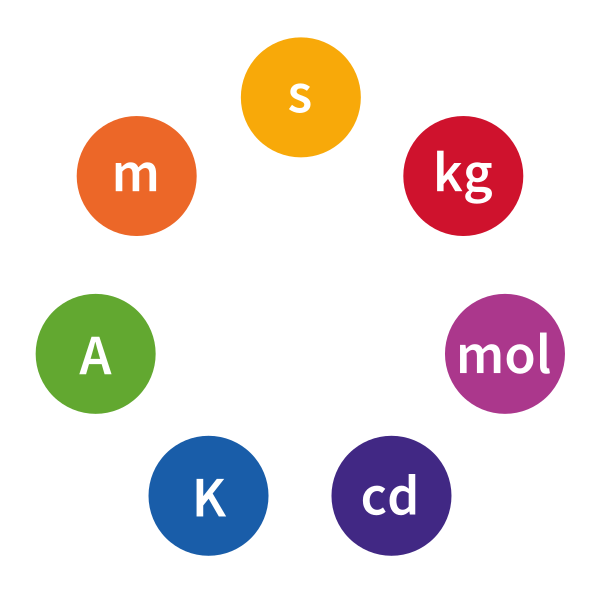
\includegraphics[width=0.5\textwidth]{SI_base_units.png}
\end{center}


(Alles andere ist abgeleitet)
\end{block}

\begin{block}{Zehnerpotenzen}

\begin{tabular}{l|l}
milli (m): \(10^{-3}\)   & kilo  (k):  \(10^{3}\)    \\
mikro (\(\mu\)): \(10^{-6}\)   & mega  (M):  \(10^{6}\)    \\
nano (n):  \(10^{-9}\)   & giga  (G):  \(10^{9}\)    \\
pico (p): \(10^{-12}\)  & tera  (T): \(10^{12}\)   \\

\end{tabular}


\end{block}




%% frequently used zehnerpotenzen

\end{column}

\begin{column}{5cm}


%% Frequently used Rechnungen
\begin{block}{Häufige Rechnungen}
\item
\textbf{Exponential}: z.B. Ansteckung 
\item
\textbf{Logarithmus}: Vereinfacht Rechnungen
\item
\textbf{Vektoren}: Werte mit Richtungen (z.B. im Raum)
\item
\textbf{Trigonometrische Funktionen}: Winkel
\item
\textbf{Differentialrechnung}: Veränderungen 
\item
\textbf{Integralrechnung}: Fläche unter einer Kurve
\end{block}



%% Frequenty used numbers

\end{column}

\end{columns}

\end{frame}


%% Fehlerrechnung

\begin{frame}{Messunsicherheit}

Abweichung zwischen echtem Wert und gemessenen Wert. \\

\begin{columns}[c]

\begin{column}{5cm}
\begin{itemize}
    \item 
Absolut: Messunsicherheit (z.B. Genauigkeit des Messgeräts)
\item
Relativ: $\frac{\text{Messunsicherheit}}{\text{gemessener Wert}}$
\end{itemize}

\end{column}

\begin{column}{5cm}
\begin{center}
    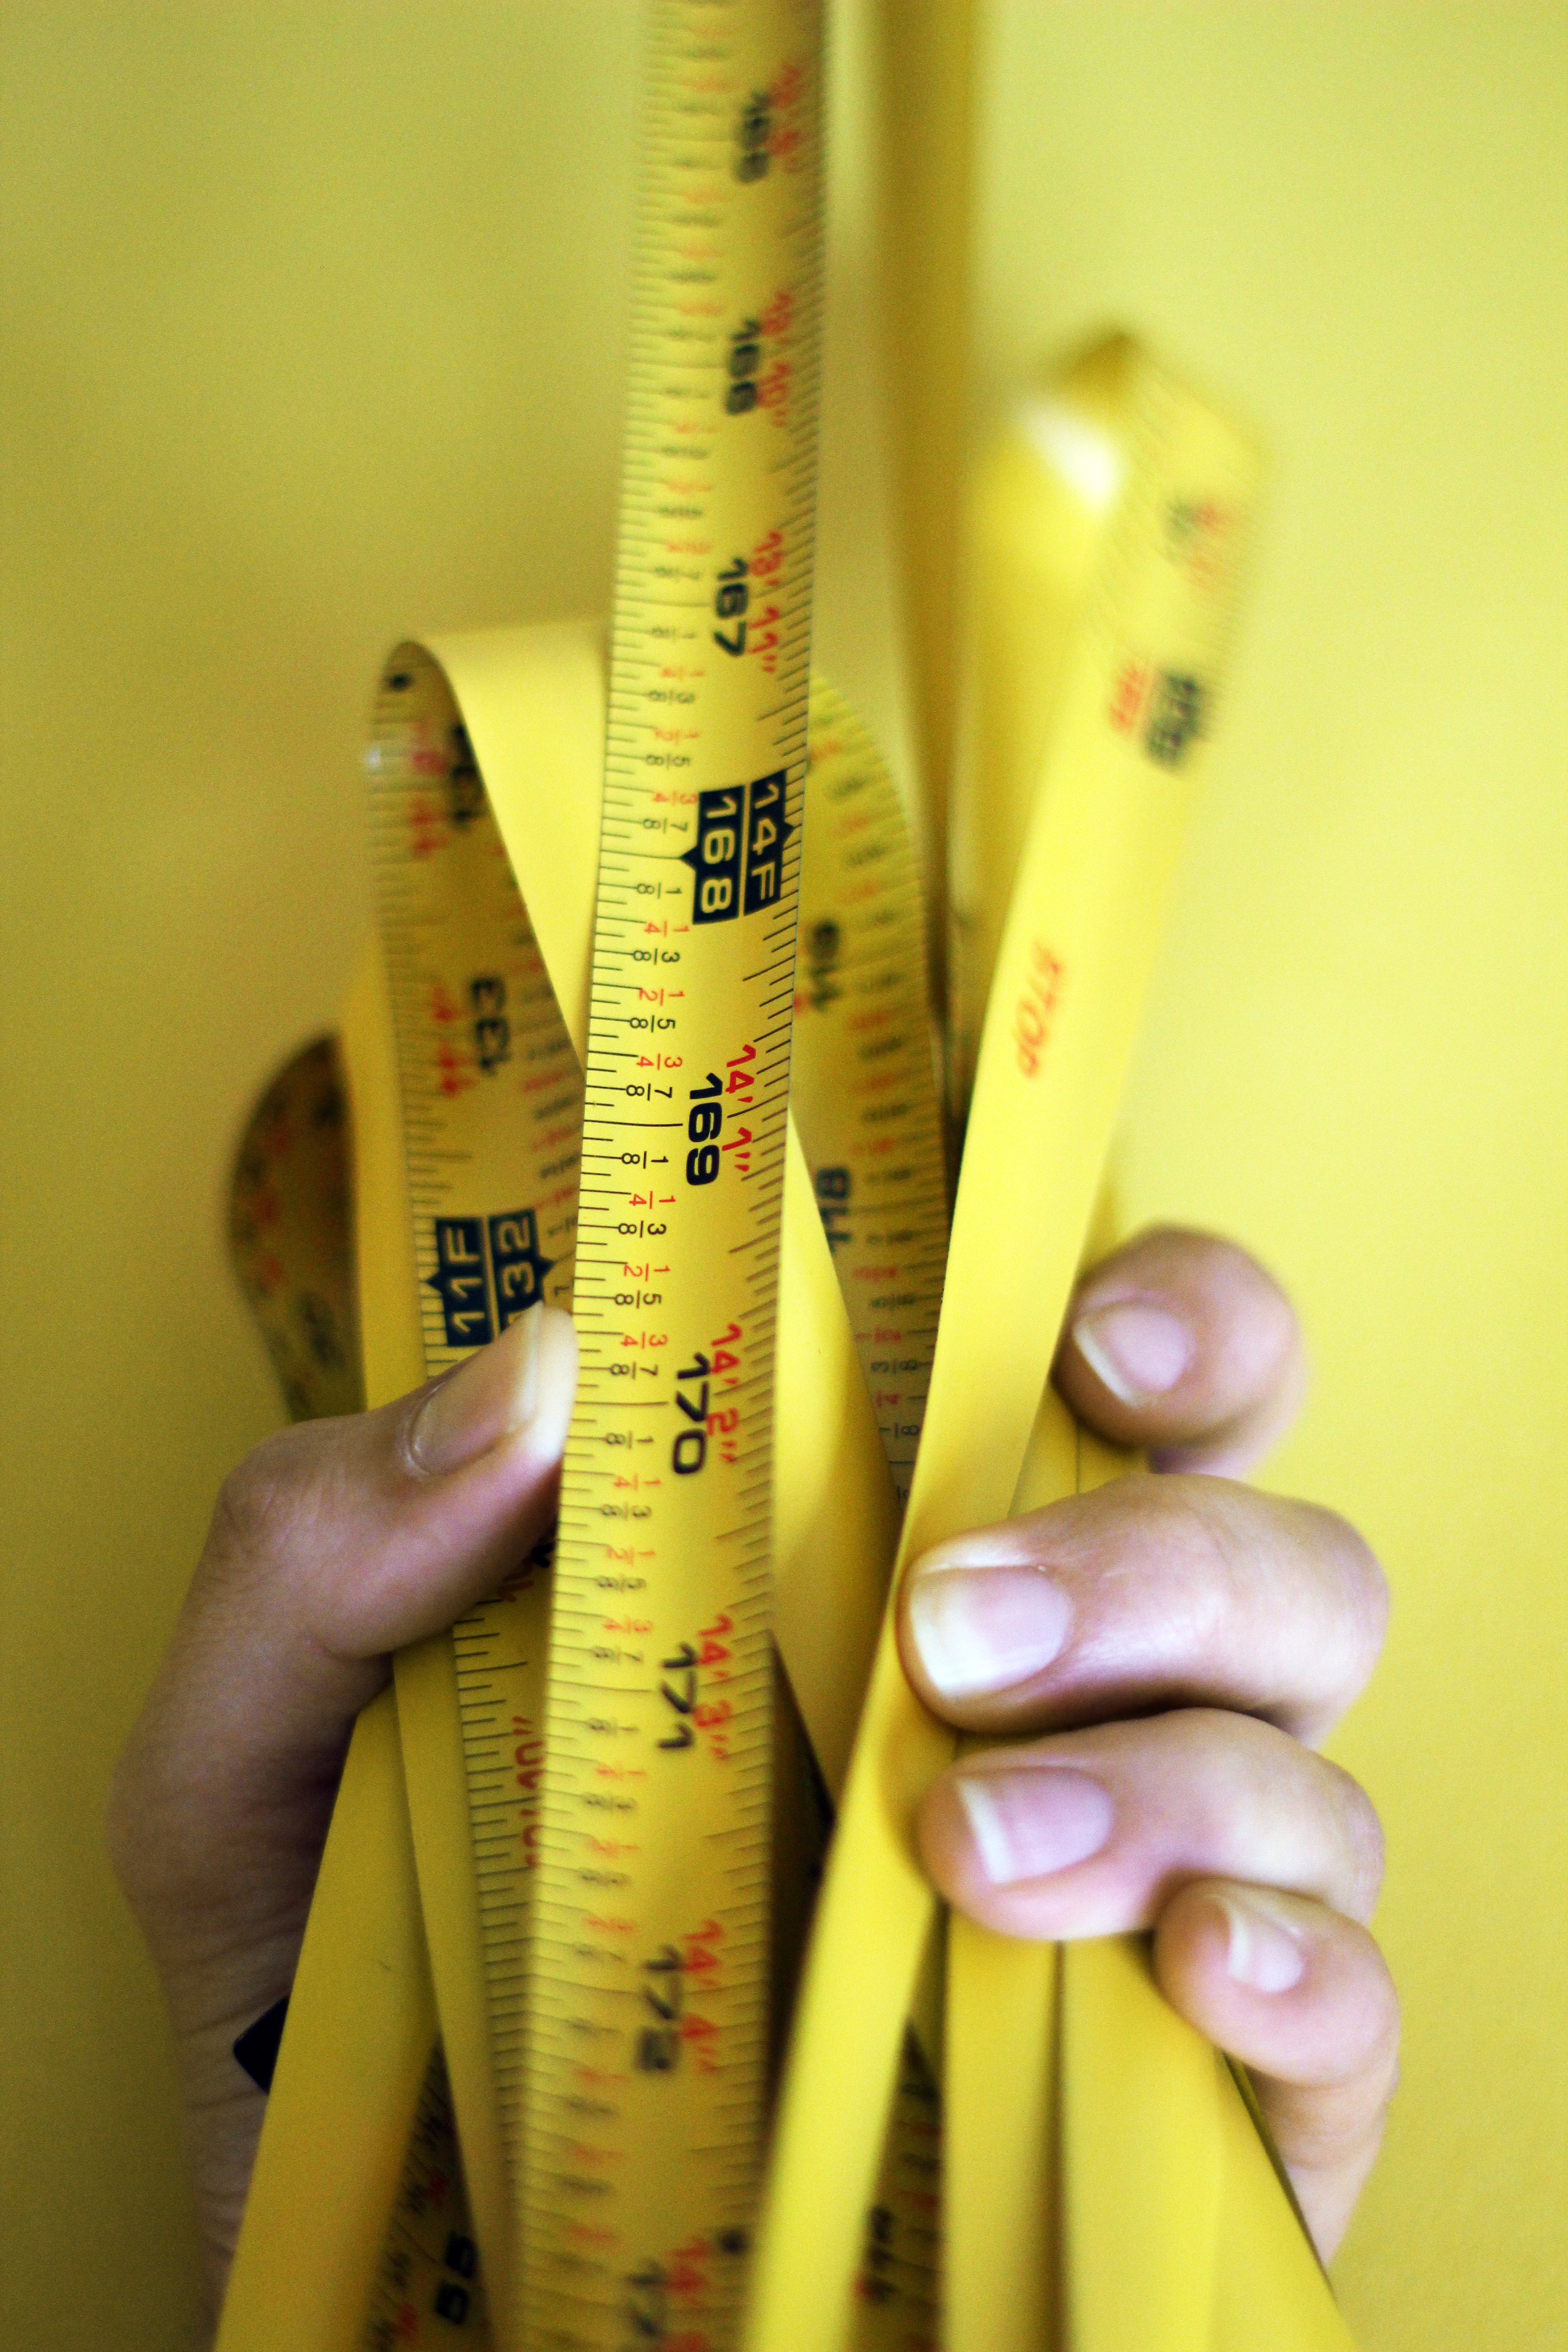
\includegraphics[width=0.6\textwidth]{massband.jpg}
\end{center}
\end{column}
\end{columns}

\pause

Fehlerfortpflanzung:

\begin{itemize}
    \item 
    Addition/Subtraktion: Die \textbf{absoluten} Unsicherheiten addieren sich.
    \item
    Multiplikation/Division: Die \textbf{relativen} Unsicherheiten addieren sich. 
\end{itemize}




% Messunsicherheit erklären
%  mit Messgrößen rechnen
%  Messunsicherheit darstellen und abschätzen
    
\end{frame}


%% Stats
\begin{frame}{Statistik}

% Mittelwert, Standardabweichung, und Standardabweichung des Mittelwerts erklären 
% Eigenschaften der Gaußschen Glockenkurve benennen
%  Mittelwert, Standardabweichung, und Standardabweichung des Mittelwerts berechnen
% verstehen, warum manche Konzepte (Gaußsche Glockenkurve, Logarithmen, Differential etc.) oft vorkommen


\begin{columns}[c]

\begin{column}{5cm}

Arithmetischer Mittelwert \\ 
(``Durchschnitt'')
\[
\bar{x} =   \frac{\sum_{i=1}^n x_i}{n}
\]

Standardabweichung \\ 
(``Schwankungsbreite'')
\[
s = \sqrt{\frac{\sum_{i=1}^n (x_i-\bar{x})^2}{n-1}}
\]

SAM (Wo kann \(\bar{x}\) sein?)
\[
SAM = \frac{s}{\sqrt{n}}
\]


\end{column}

\pause
\begin{column}{6cm}

\begin{block}{Normalverteilung }
Gaußsche Glockenkurve

Kommt oft vor (Bsp. Körpergröße)

"68–95–99.7 Regel"

\begin{center}
    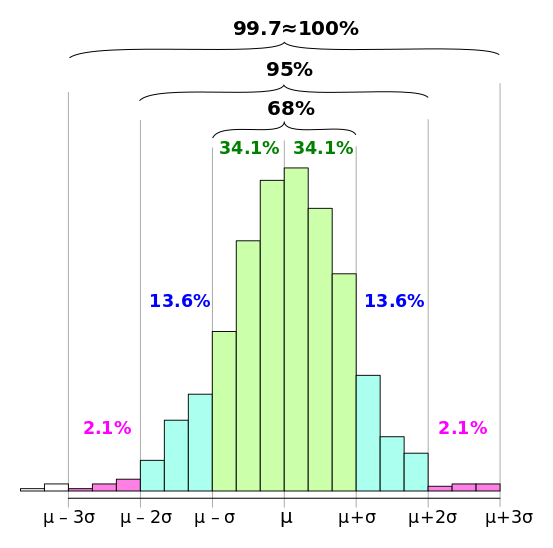
\includegraphics[width=\textwidth]{Empirical_rule_histogram.png}
\end{center}


\end{block}

\end{column}


\end{columns}



    
\end{frame}



%% Methodik IMPP Fragen


% %% Würfel
\begin{frame}{IMPP-Fragen zu M01.1}

\textbf{Würfelförmige Zellen mit jeweils \(10\,\mu m\) Kantenlänge  bilden mit vernachlässigbar kleinen Zwischenräumen ein Gewebe.}

\textbf{Wie viele Zellen sind in \(1\,cm^3 \) eines derartigen Gewebes enthalten?} \\[0.2 cm]

\begin{description}
\item{A.}
1000
\item{B.}
1 Million
\item{C.}
1 Milliarde %% correct
\item{D.}
100 Milliarden
\item{E.}
1 Billion
\end{description}

    
\end{frame}

\begin{frame}{IMPP-Fragen zu M01.1}

\textbf{Würfelförmige Zellen mit jeweils \(10\,\mu m\) Kantenlänge  bilden mit vernachlässigbar kleinen Zwischenräumen ein Gewebe.}

\textbf{Wie viele Zellen sind in \(1\,cm^3 \) eines derartigen Gewebes enthalten?} \\[0.2 cm]


Wie viele Zellen pro Kante? 



\begin{columns}[t]


\begin{column}{5cm}
%% pictures from iphone
\includegraphics<1>[width=\textwidth]{Gewebe_Wuerfel.jpeg}
\includegraphics<2->[width=\textwidth]{Zellen.jpeg}
\end{column}

\pause
\begin{column}{6cm}
%% pictures from iphone

\pause

\[1\,cm = 10^{-2}\,m\]

\[10\,\mu m = 10^{-5}\,m\]

\[
\frac {10^{-2}}{10^{-5}} = 10^{-2-(-5)} = 10^3
 \]

\pause
Volumen = Länge \(\times\) Breite \(\times\) Höhe 


\end{column}

\end{columns}

\end{frame}

\begin{frame}{IMPP-Fragen zu M01.1}

\textbf{Würfelförmige Zellen mit jeweils \(10\,\mu m\) Kantenlänge  bilden mit vernachlässigbar kleinen Zwischenräumen ein Gewebe.}

\textbf{Wie viele Zellen sind in \(1\,cm^3 \) eines derartigen Gewebes enthalten?} \\[0.2 cm]


Wie viele Zellen pro Kante? 



\begin{columns}[c]

\begin{column}{5cm}
%% pictures from iphone
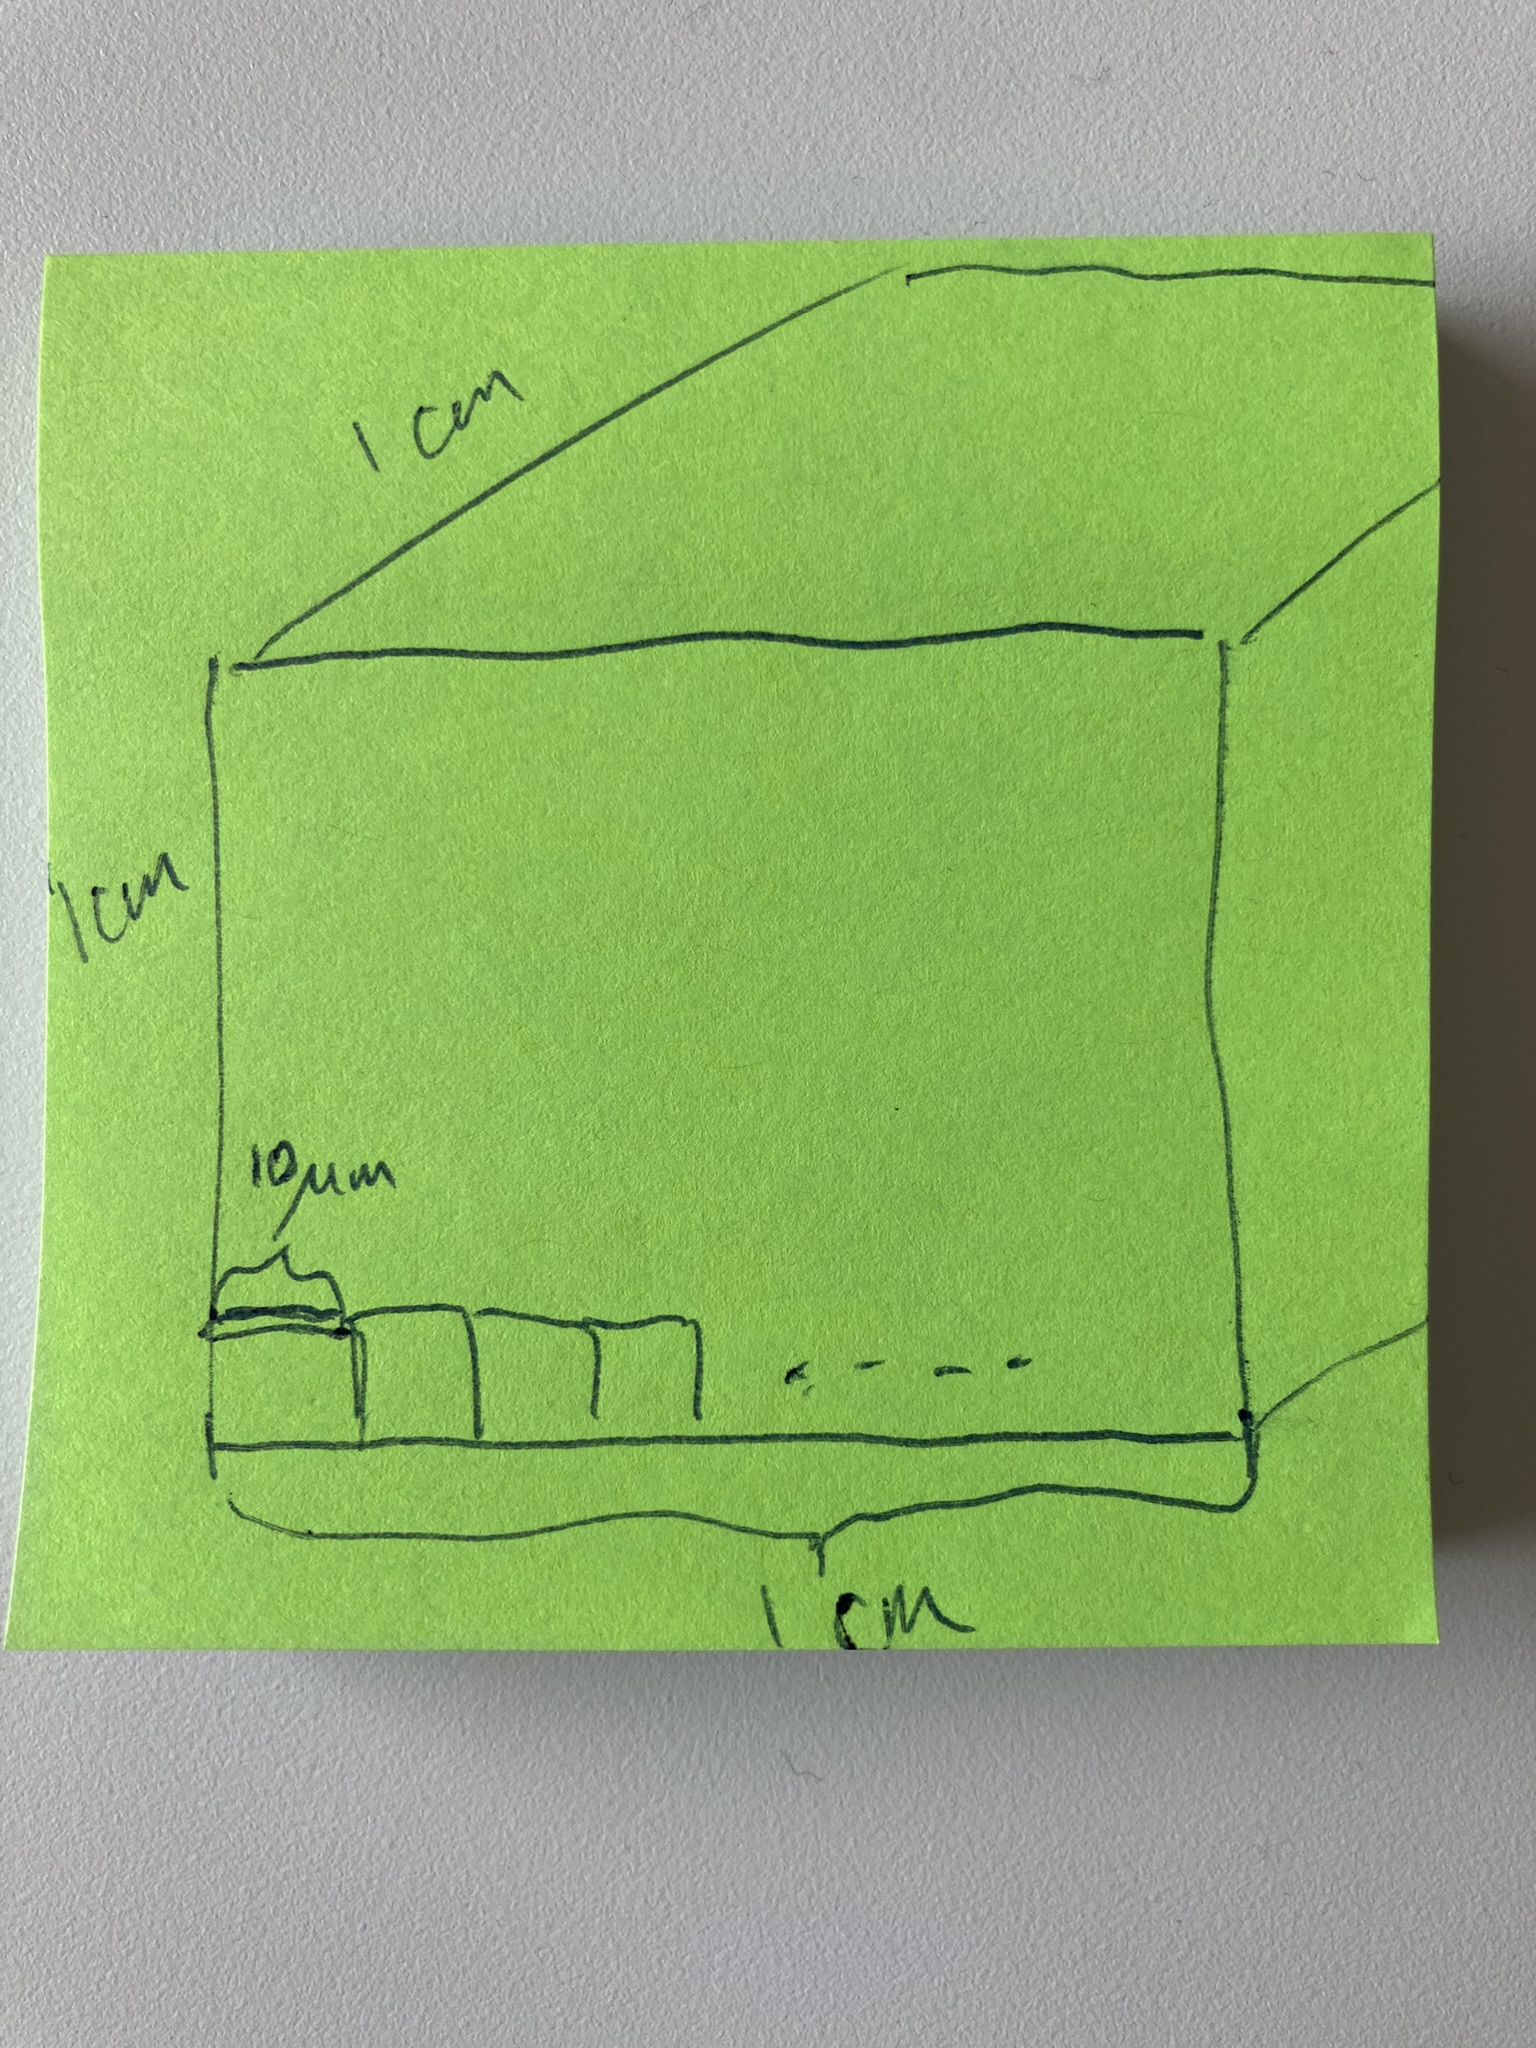
\includegraphics[width=\textwidth]{Zellen.jpeg}
\end{column}

\begin{column}{6cm}
%% pictures from iphone
\[1\,cm = 10^{-2}\,m\]

\[10\,\mu m = 10^{-5}\,m\]

\[
\frac {10^{-2}}{10^{-5}} = 10^{-2-(-5)} = 10^3
 \]

Volumen = \(10^3 \times 10^3 \times 10^3 = 10^9 = 1\, \text{Milliarde} \)

\end{column}

\end{columns}

\end{frame}





\begin{frame}{IMPP-Fragen zu M01.1}

\textbf{Würfelförmige Zellen mit jeweils \(10\,\mu m\) Kantenlänge  bilden mit vernachlässigbar kleinen Zwischenräumen ein Gewebe.}

\textbf{Wie viele Zellen sind in \(1\,cm^3 \) eines derartigen Gewebes enthalten?} \\[0.2 cm]

\begin{description}
\item{A.}
1000
\item{B.}
1 Million
\item{C.} 
\textcolor{theme}{\textbf{1 Milliarde}}
\item{D.}
100 Milliarden
\item{E.}
1 Billion
\end{description}

    
\end{frame}


% %% Messfehler

\begin{frame}{IMPP-Fragen zu M01.1}
\textbf{Die Messunsicherheit eines Blutdruckmessgeräts wird in der Bedienungsanleitung mit \(\pm 3\, mmHg\) angegeben. Bei einer Messung wird als diastolischer Wert \(90\,mmHg\) angezeigt.}

\textbf{Etwa wie groß ist somit die relative Messunsicherheit dieses Wertes (wenn die Angabe in der Bedienungsanleitung zutrifft)?}\\[0.2 cm]


\begin{description}
\item[A]
\(\pm 0,2\,\%\) 
\item[B]
\(\pm 0,3\,\%\) 
\item[C] 
\(\pm 0,9\,\% \) 
\item[D]
\(\pm 2\,\%\) 
\item[E]
\(\pm 3\,\%\) 
\end{description}
    
\end{frame}


\begin{frame}{IMPP-Fragen zu M01.1}

\textbf{Die Messunsicherheit eines Blutdruckmessgeräts wird in der Bedienungsanleitung mit \(\pm 3\, mmHg\) angegeben. Bei einer Messung wird als diastolischer Wert \(90\,mmHg\) angezeigt.}

\textbf{Etwa wie groß ist somit die relative Messunsicherheit dieses Wertes (wenn die Angabe in der Bedienungsanleitung zutrifft)?}\\[0.2 cm]


Relative Messunsicherheit = \(\frac{\text{absolute Messunsicherheit}}{\text{gemessener Wert}}\)

\[
\frac{3\,mmHg}{90\,mmHg} \approx 0.03 = 3\,\%
\]


\end{frame}


\begin{frame}{IMPP-Fragen zu M01.1}
\textbf{Die Messunsicherheit eines Blutdruckmessgeräts wird in der Bedienungsanleitung mit \(\pm 3\, mmHg\) angegeben. Bei einer Messung wird als diastolischer Wert \(90\,mmHg\) angezeigt.}

\textbf{Etwa wie groß ist somit die relative Messunsicherheit dieses Wertes (wenn die Angabe in der Bedienungsanleitung zutrifft)?}\\[0.2 cm]


\begin{description}
\item{A.}
\(\pm 0,2\,\%\) 
\item{B.}
\(\pm 0,3\,\%\) 
\item{C.} 
\(\pm 0,9\,\% \) 
\item{D.}
\(\pm 2\,\%\) 
\item{E.}
\textcolor{theme}{\(\pm 3\,\%\) }
\end{description}
    
\end{frame}



% %% Männer

\begin{frame}{IMPP-Fragen zu M01.1}

\textbf{Bei einer großen Anzahl männlicher Probanden wurde eine Reihenuntersuchung durchgeführt. Es ergab sich für die Körpergröße eine (Gauß-) Normalverteiling mit einem Mittelwert von \(1,80\,m\) und einer Standardabwichung von \(10\,cm\) }

\textbf{Welche Aussage zur Größenverteilung dieser Männer trifft am ehesten zu? }\\[0.2 cm]

\begin{description}
\item[A]
Etwa \(5\,\%\) sind mindestens \(2\,m\) groß
\item[B]
Etwa \(16\,\%\) sind höchstens \(1,50 \, m\) groß
\item[C] 
Etwa \(32\,\% \) sind zwischen \(1,70\,m\) und \(1,90\,m\) groß

\item[D]
Etwa \(50\,\%\) sind mindestens \(1,80\,m\) groß
\item[E]
Etwa  \(68\,\%\) sind höchstens \(1,90\,m\) groß
\end{description}

    
\end{frame}



\begin{frame}{IMPP-Fragen zu M01.1}

\textbf{Bei einer großen Anzahl männlicher Probanden wurde eine Reihenuntersuchung durchgeführt. Es ergab sich für die Körpergröße eine (Gauß-) Normalverteiling mit einem Mittelwert von \(1,80\,m\) und einer Standardabwichung von \(10\,cm\) }

\textbf{Welche Aussage zur Größenverteilung dieser Männer trifft am ehesten zu? }\\[0.2 cm]

68-95-99.7-Regel: 

\begin{itemize}
    \item 
    \(68\,\%\) sind zwischen  \(1,70\,m\) und \(1,90\,m\) \\(Mittelwert \(\pm\) 1 Standardabweichung)
    \item 
    \(95\,\%\) sind zwischen  \(1,60\,m\) und \(2,00\,m\)
    \item 
    \(99.7\,\%\) sind zwischen  \(1,50\,m\) und \(2,10\,m\)

\end{itemize}

Damit muss man sich die einzelnen Antworten durchüberlegen. \pause Oder?

\end{frame}


\begin{frame}{IMPP-Fragen zu M01.1}

Oder einfacher: Die Gaußsche Glockenkurve ist symmetrisch!

\begin{center}
    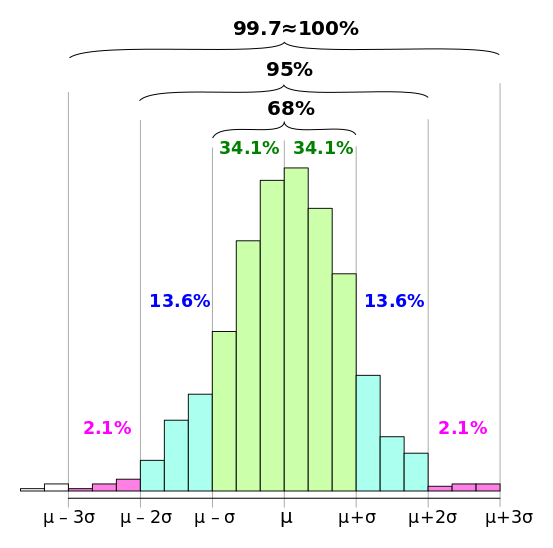
\includegraphics[width=0.5\textwidth]{Empirical_rule_histogram.png}
\end{center}

Daher ca. gleich viele Werte unter dem Mittelwert wie drüber


\end{frame}

\begin{frame}{IMPP-Fragen zu M01.1}

\textbf{Bei einer großen Anzahl männlicher Probanden wurde eine Reihenuntersuchung durchgeführt. Es ergab sich für die Körpergröße eine (Gauß-) Normalverteiling mit einem Mittelwert von \(1,80\,m\) und einer Standardabwichung von \(10\,cm\) }

\textbf{Welche Aussage zur Größenverteilung dieser Männer trifft am ehesten zu? }\\[0.2 cm]

\begin{description}
\item[A]
Etwa \(5\,\%\) sind mindestens \(2\,m\) groß
\item[B]
Etwa \(16\,\%\) sind höchstens \(1,50 \, m\) groß
\item[C] 
Etwa \(32\,\% \) sind zwischen \(1,70\,m\) und \(1,90\,m\) groß

\item[D]
\textcolor{theme}{Etwa \(50\,\%\) sind mindestens \(1,80\,m\) groß}
\item[E]
Etwa  \(68\,\%\) sind höchstens \(1,90\,m\) groß
\end{description}

    
\end{frame}




\section{M01.2 Mechanik}


%% Learning Objectives 


% \begin{block}{Wissen:}
% \begin{itemize}
% \item
% Zusammenhang zwischen Strecke, Geschwindigkeit und Beschleunigung erklären
% \item
% Periodendauer, Frequenz und Kreisfrequenz definieren
% \item
% die Newtonschen Axiome nennen
% \item
% Impuls und Kraft definieren
% \item
% den  Impulserhaltungssatz wiedergeben und Beispiele geben
% \item
% Arbeit, Leistung und Energie definieren
% \item
% Arten von Energie unterscheiden
% \item
% den Energieerhaltungssatz erklären
% \item
% Drehmoment definieren und das Hebelgesetz
% \item
% Trägheitsmoment und Drehimpuls definieren
% \item
% den Drehimpulserhaltungssatz erklären und Beispiele nennen 
% \end{itemize}

% \end{block}

% \end{frame}

% \begin{frame}

% \frametitle{Nach dieser Vorlesung sollten Sie:}
 



% \begin{block}{Können:}
% \begin{itemize}
% \item
% Bewegungsdiagramme lesen und verstehen/auswerten
% \item
% Mittelwert und Momentanwert der Geschwindigkeit errechnen
% \item
% Parameter einer Kreisbewegung berechnen
% \item 
% das Hebelgesetz anwenden
% \end{itemize}
% \end{block}


 
% \begin{block}{Fühlen:}
% \begin{itemize}
% \item
% mechanische Prozesse im täglichen Leben erkennen
% \item
% über Anwendungen von Mechanik in der Medizin nachdenken
% \end{itemize}
% \end{block}

%  \end{frame}



%% Slides


%% Bewegung, Kraft ,Impuls

\begin{frame}{Bewegung, Kraft, Impuls}
    
\begin{columns}[c]



\begin{column}{6cm}
    \begin{block}{Geschwindigkeit, Beschleunigung}
    Geschwindigkeit v: Weg/Zeit \\  

\begin{center}
    %% Pictures post-its winkel, bahn, gerade
    \includegraphics<1>[width=0.6\textwidth]{gerade.jpeg}
    \includegraphics<2>[width=0.6\textwidth]{Greade_kreis.jpeg}
    \includegraphics<3->[width=0.6\textwidth]{winkelgeschwindigkeit.jpeg}
\end{center}



\end{block}




\end{column}

\begin{column}{5cm}



\end{column}


\end{columns}

    
    
    
\end{frame}




\begin{frame}{Bewegung, Kraft, Impuls}
    
\begin{columns}[c]



\begin{column}{6cm}
    \begin{block}{Geschwindigkeit, Beschleunigung}
    Geschwindigkeit v: Weg/Zeit \\  



    \pause
    Beschleunigung a: Geschwindikgeit/Zeit
        \end{block}

\pause

\begin{block}{Kraft, Impuls}
Kraft: Masse \(\times\) Beschleunigung \\
Einheit: \( kg\times\frac{m}{s^2} = N \) \\[0.2cm]
\pause
Impuls: Masse \(\times\) Geschwindikgeit \\
Einheit: \( kg\times\frac{m}{s} \)


\end{block}




\end{column}

\begin{column}{5cm}


\begin{block}{Erhaltungssätze}
Newtonsche Axiome: \\
1. Ein kräftefreier Körper bleibt in Ruhe oder bewegt sich geradlinig mit konstanter Geschwindigkeit. \\
2. Kraft = Masse mal Beschleunigung \\
3. Kraft = Gegenkraft \\[0.2 cm]
\pause
Impulserhaltung: In einem geschlossenen System bleibt der Gesamtimpuls gleich \\(bis auf Reibung)


\end{block}

%% Erhaltungssätze

% Newtonsche Axiome
%% Impuls + Impulserhaltung

\end{column}


\end{columns}

    
    
    
\end{frame}



%% Arbeit, Energie, Leistung

\begin{frame}{Arbeit, Energie, Leistung}
    
    \begin{columns}
\begin{column}{5cm}
Arbeit = Kraft  mal Weg \\
Einheit: Newton\(\times\)meter (Nm) = Joule (J)  \\
\pause
Leistung = Arbeit pro Zeit \\

%% Bergweg

\includegraphics[width=\textwidth]{bergweg.jpg}


\end{column}    
\pause


\begin{column}{5cm}
Energie = gespeicherte Arbeit \\


\begin{itemize}
\item
Bewegungsenergie 
\item
Lageenergie 
\item
Verformungsenergie
\item
Thermische Energie
\item
Chemische Energie
\item
Elektrische Energie
\end{itemize}

Energierhaltung: Arten von Energie können ineinander umgewandelt werden, aber die Gesamtenergie in einem geschlossenen System ist konstant. 

\end{column}    

    \end{columns}
    
\end{frame}

%% Drehmoment, Trägheitsmoment, Drehimpuls

\begin{frame}{Drehmoment, Trägheitsmoment, Drehimpuls}

\begin{columns}[c]

\begin{column}{5cm}
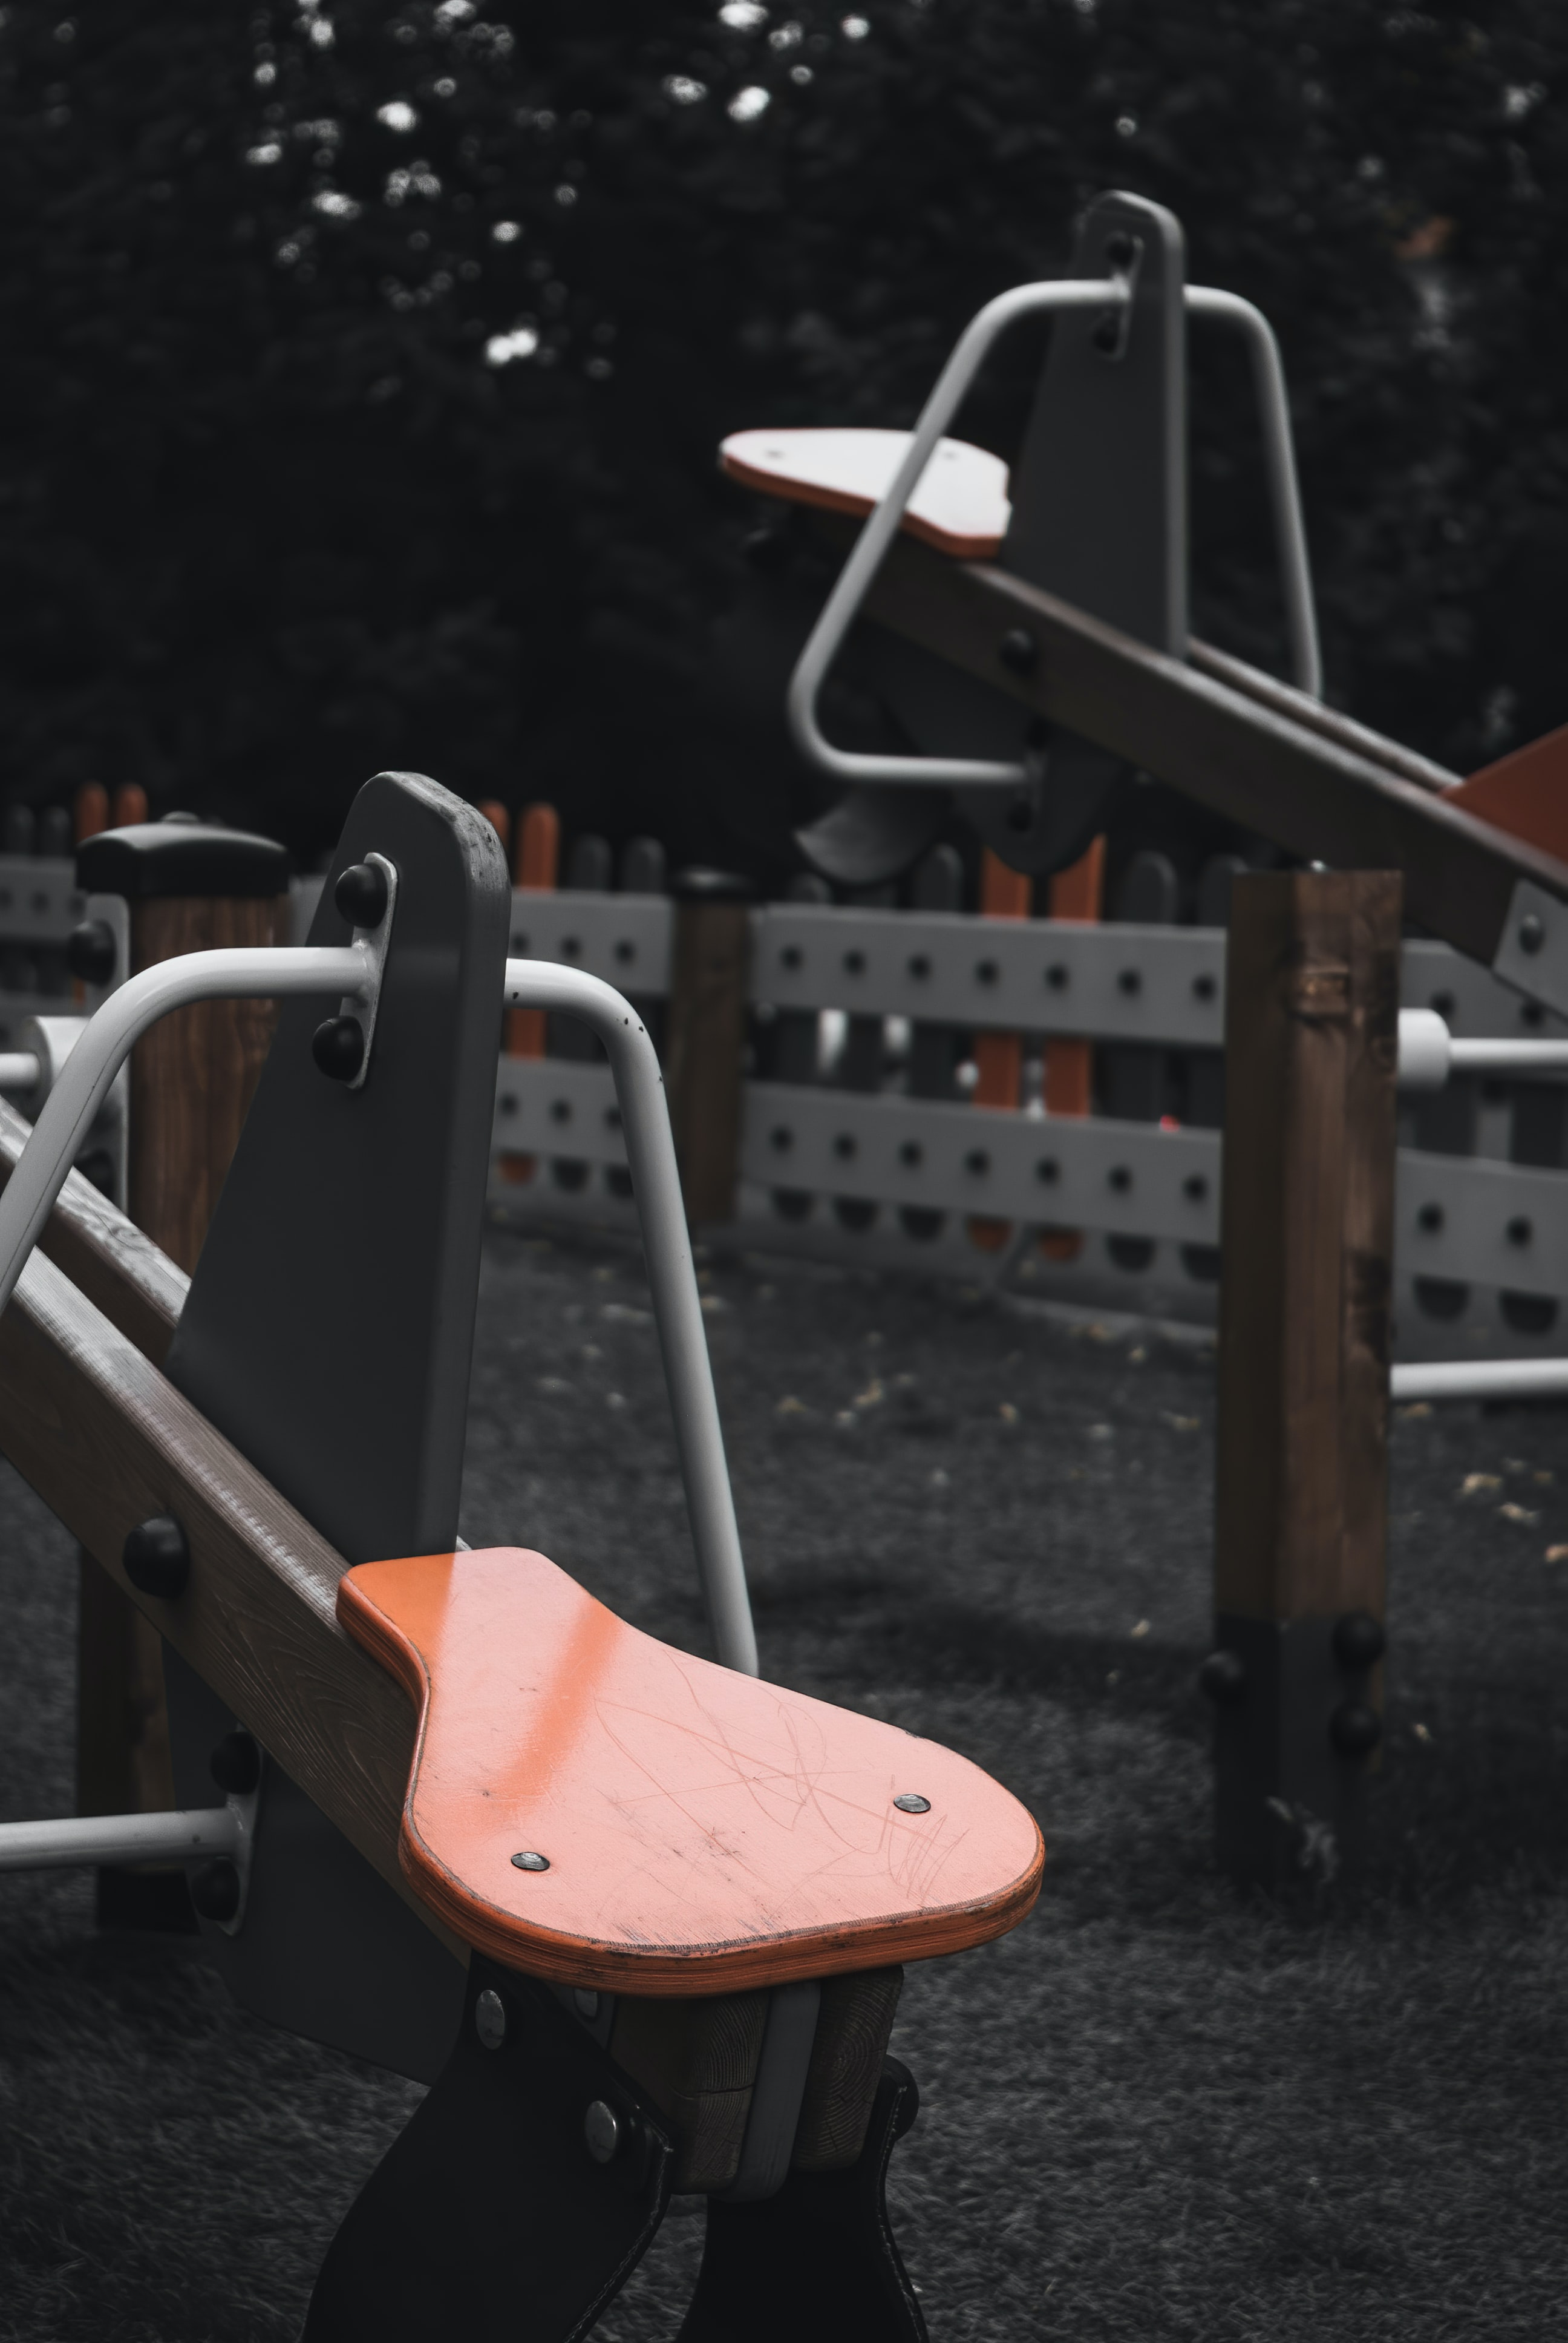
\includegraphics[width=\textwidth]{wippen.jpg}

\end{column}


\begin{column}{6cm}

Drehmoment = Kraft mal Länge des Hebelarms

Hebelgesetz: \\
Kraft \times Kraftarm = Last \times Lastarm 

\pause

Trägheitsmoment: Trägheit gegenüber Veränderungen in der Winkelgeschwindigkeit (hängt von Verteilung der Masse ab: je mehr Masse weiter weg von der Drehachse, desto größer das Trägheitsmoment)

\pause

Drehimpuls: Trägheitsmoment mal Winkelgeschwindigkeit 

\pause

Drehimpulserhaltung: Der Drehimpuls bleibt  erhalten (bis auf Reibungsverluste)

\end{column}



\end{columns}



\end{frame}



%% IMPP Fragen

%% Boxer (Bewegung, Kraft, Impuls)
 
\begin{frame}{IMPP-Fragen zu M01.2}
    
    \textbf{Der Kopf eines Boxers wird durch einen Faustschlag getroffen. Der Kopf wird vereinfacht als isolierter, zentral getroffener und mit einer Kraft von \(3\,000\,N\) beschleunigter Körper der Masse \(5\,kg\) betrachtet.}
    
   \textbf{ Etwa wievielmal größer als die Erdbeschleunigung g ist die Beschleunigung, die der Kopf somit erhält?    } \\[0.2cm]
    
    

\begin{columns}[c]
\begin{column}{5cm}

    \begin{description}
    \item{A.} 60-mal    % correct
    \item{B.} 150-mal
    \item{C.} 600-mal
    \item{D.} 1\,500-mal
    \item{E.} 15\,000-mal
    \end{description}

    \end{column}

    \begin{column}{5cm}

\begin{center}
    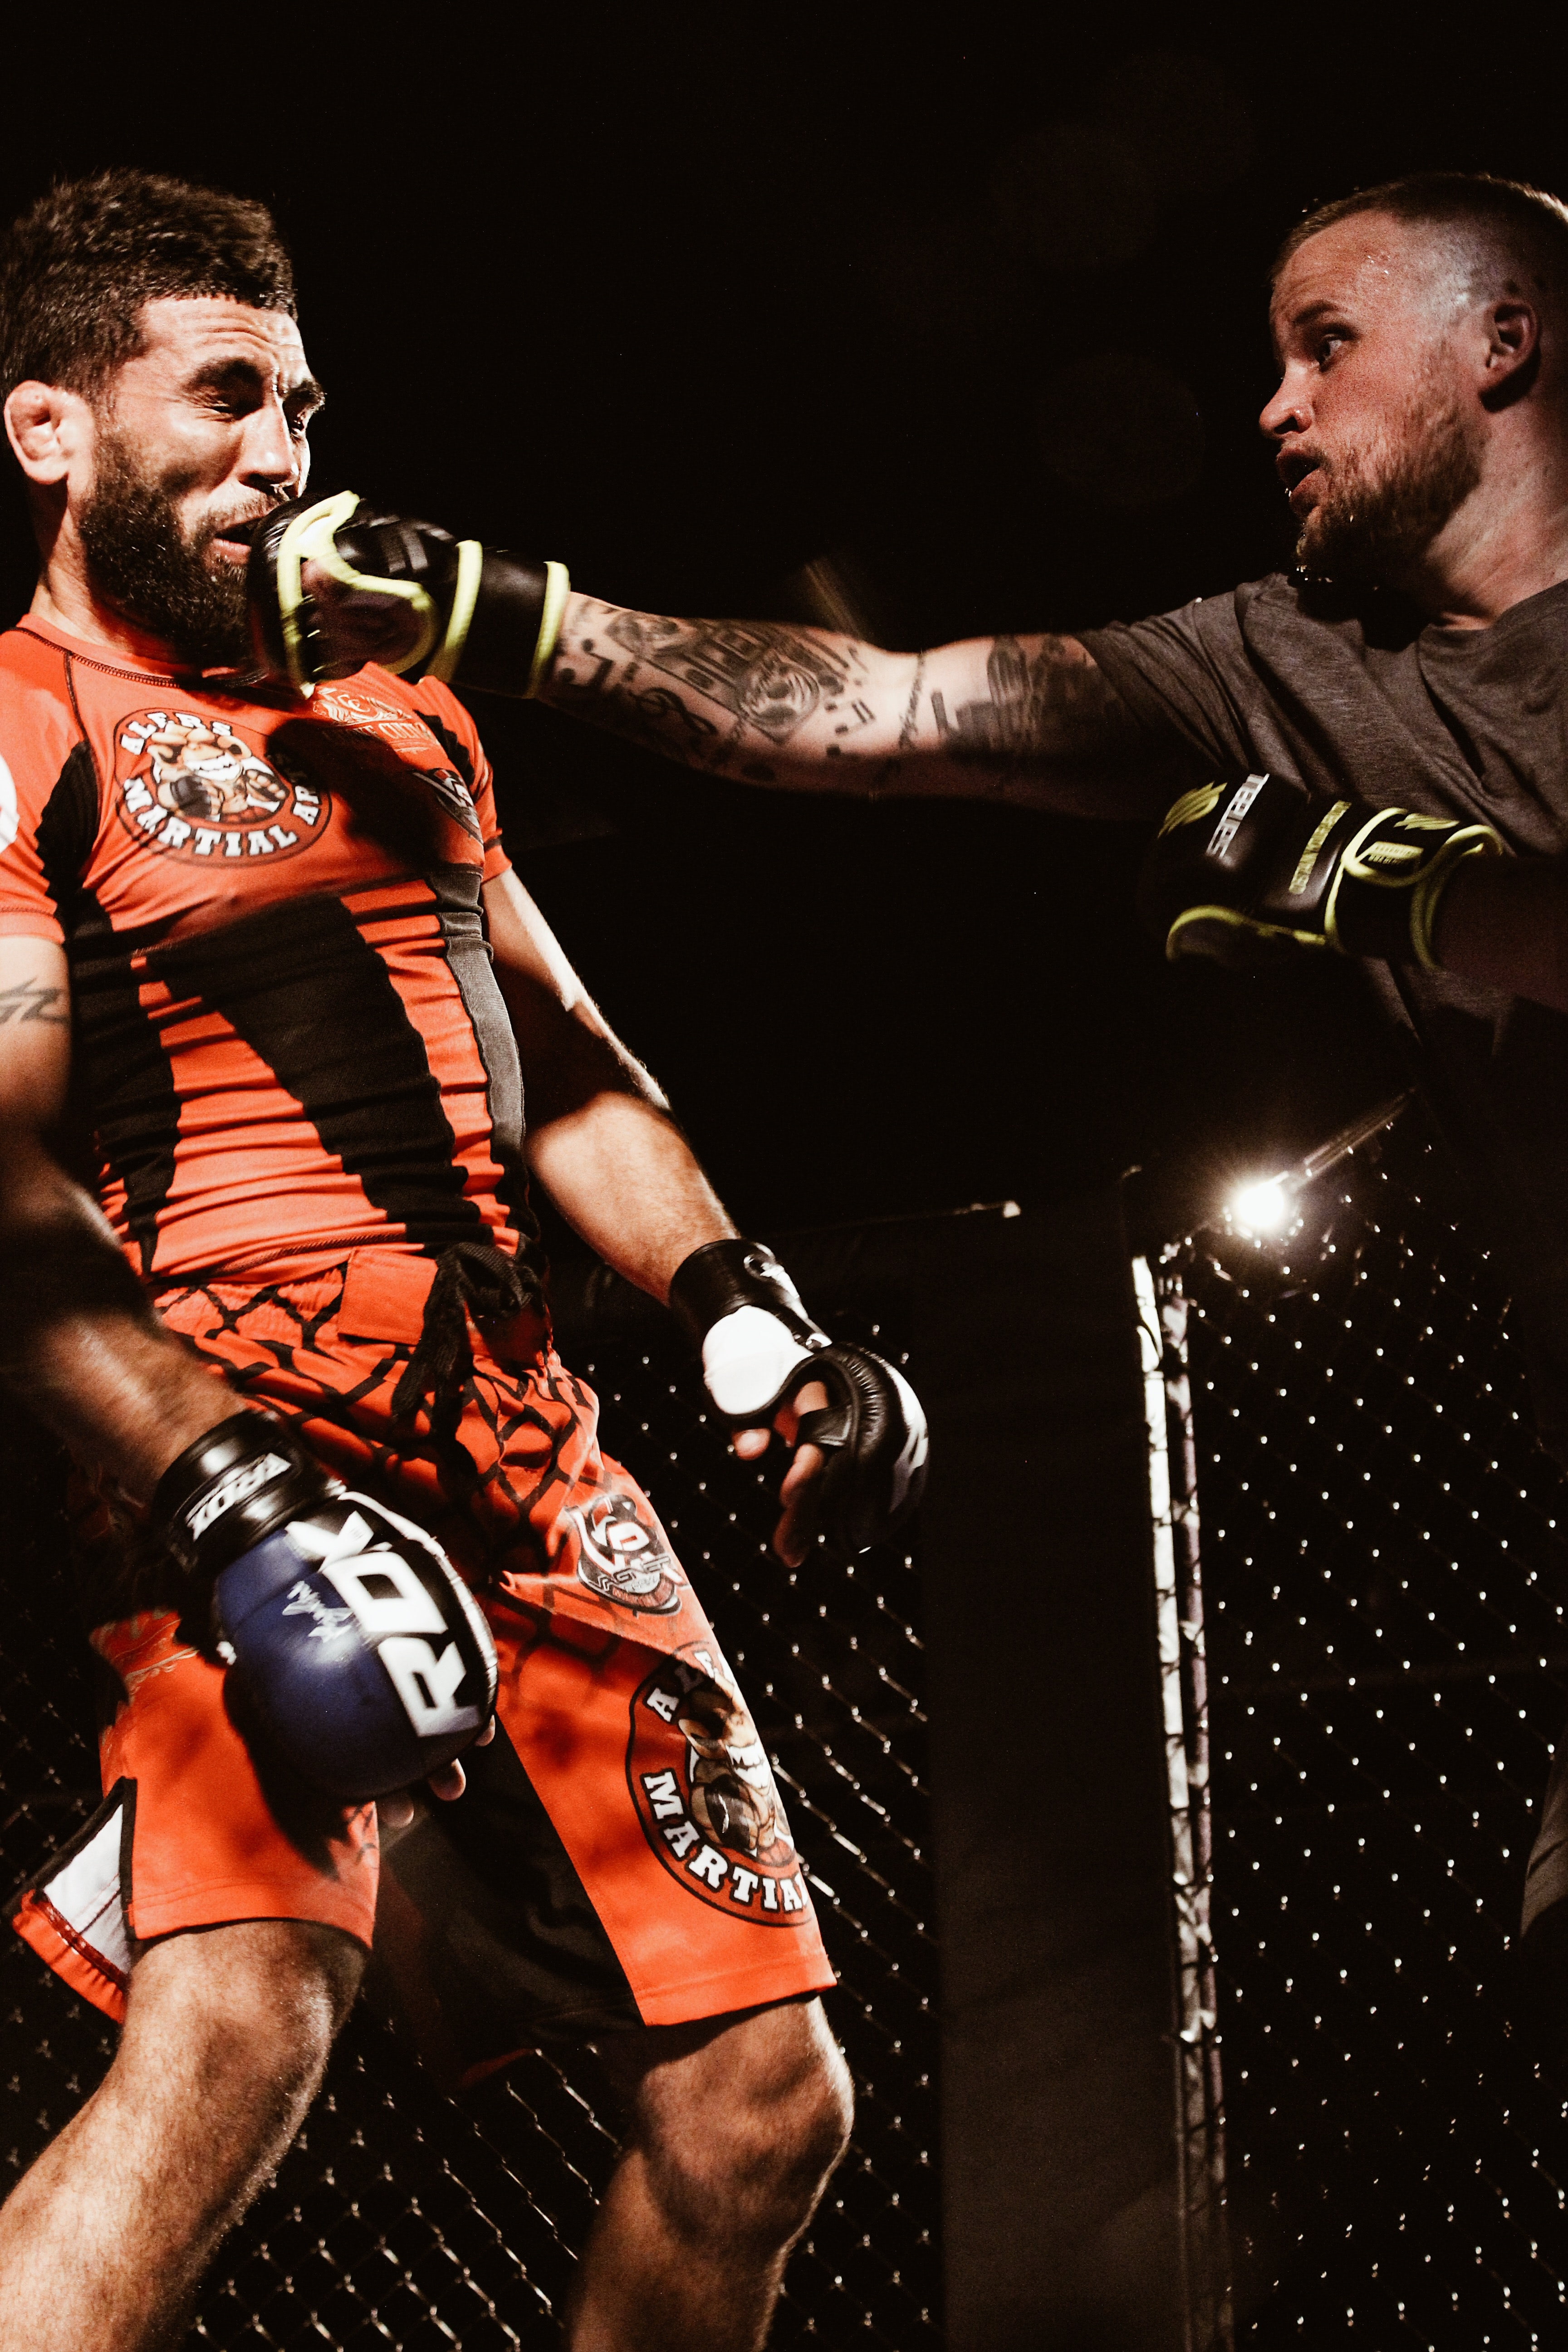
\includegraphics[width=0.6\textwidth]{boxer.jpg}
\end{center}
    
    \end{column}

    
    \end{columns}
    
\end{frame}



\begin{frame}{IMPP-Fragen zu M01.2}
    
    \textbf{Der Kopf eines Boxers wird durch einen Faustschlag getroffen. Der Kopf wird vereinfacht als isolierter, zentral getroffener und mit einer Kraft von \(3\,000\,N\) beschleunigter Körper der Masse \(5\,kg\) betrachtet.}
    
        \textbf{Etwa wievielmal größer als die Erdbeschleunigung g ist die Beschleunigung, die der Kopf somit erhält?    } \\[0.2cm]


Wir brauchen:  Beschleunigung. \pause Wir haben:  Masse und Kraft. \\

\pause
\[
F = m\times a
\]

\[
a = \frac{F}{m} \pause   = \frac{3000\,N}{5\,kg} = \pause \frac{3000\,kg\, m\, s^{-2}}{5\,kg} = 600\,\frac{m}{s^2}
  \]
  
  \pause
   
  Was war die Erdbeschleunigung? \pause \(g= 10\,\frac{m}{s^2}\)  \\
  \pause
  Wieviel mal größer?  \(\frac{600}{10} = 60\)
 

\end{frame}



\begin{frame}{IMPP-Fragen zu M01.2}
    
    \textbf{Der Kopf eines Boxers wird durch einen Faustschlag getroffen. Der Kopf wird vereinfacht als isolierter, zentral getroffener und mit einer Kraft von \(3\,000\,N\) beschleunigter Körper der Masse \(5\,kg\) betrachtet.}
    
\textbf{    Etwa wievielmal größer als die Erdbeschleunigung g ist die Beschleunigung, die der Kopf somit erhält?    } \\[0.2cm]
    
    

\begin{columns}[c]
\begin{column}{5cm}

    \begin{description}
    \item{A.} \textbf{\textcolor{theme}{60-mal} }
    \item{B.} 150-mal
    \item{C.} 600-mal
    \item{D.} 1\,500-mal
    \item{E.} 15\,000-mal
    \end{description}
    
    
    

    
    \end{column}

    \begin{column}{5cm}

\begin{center}
    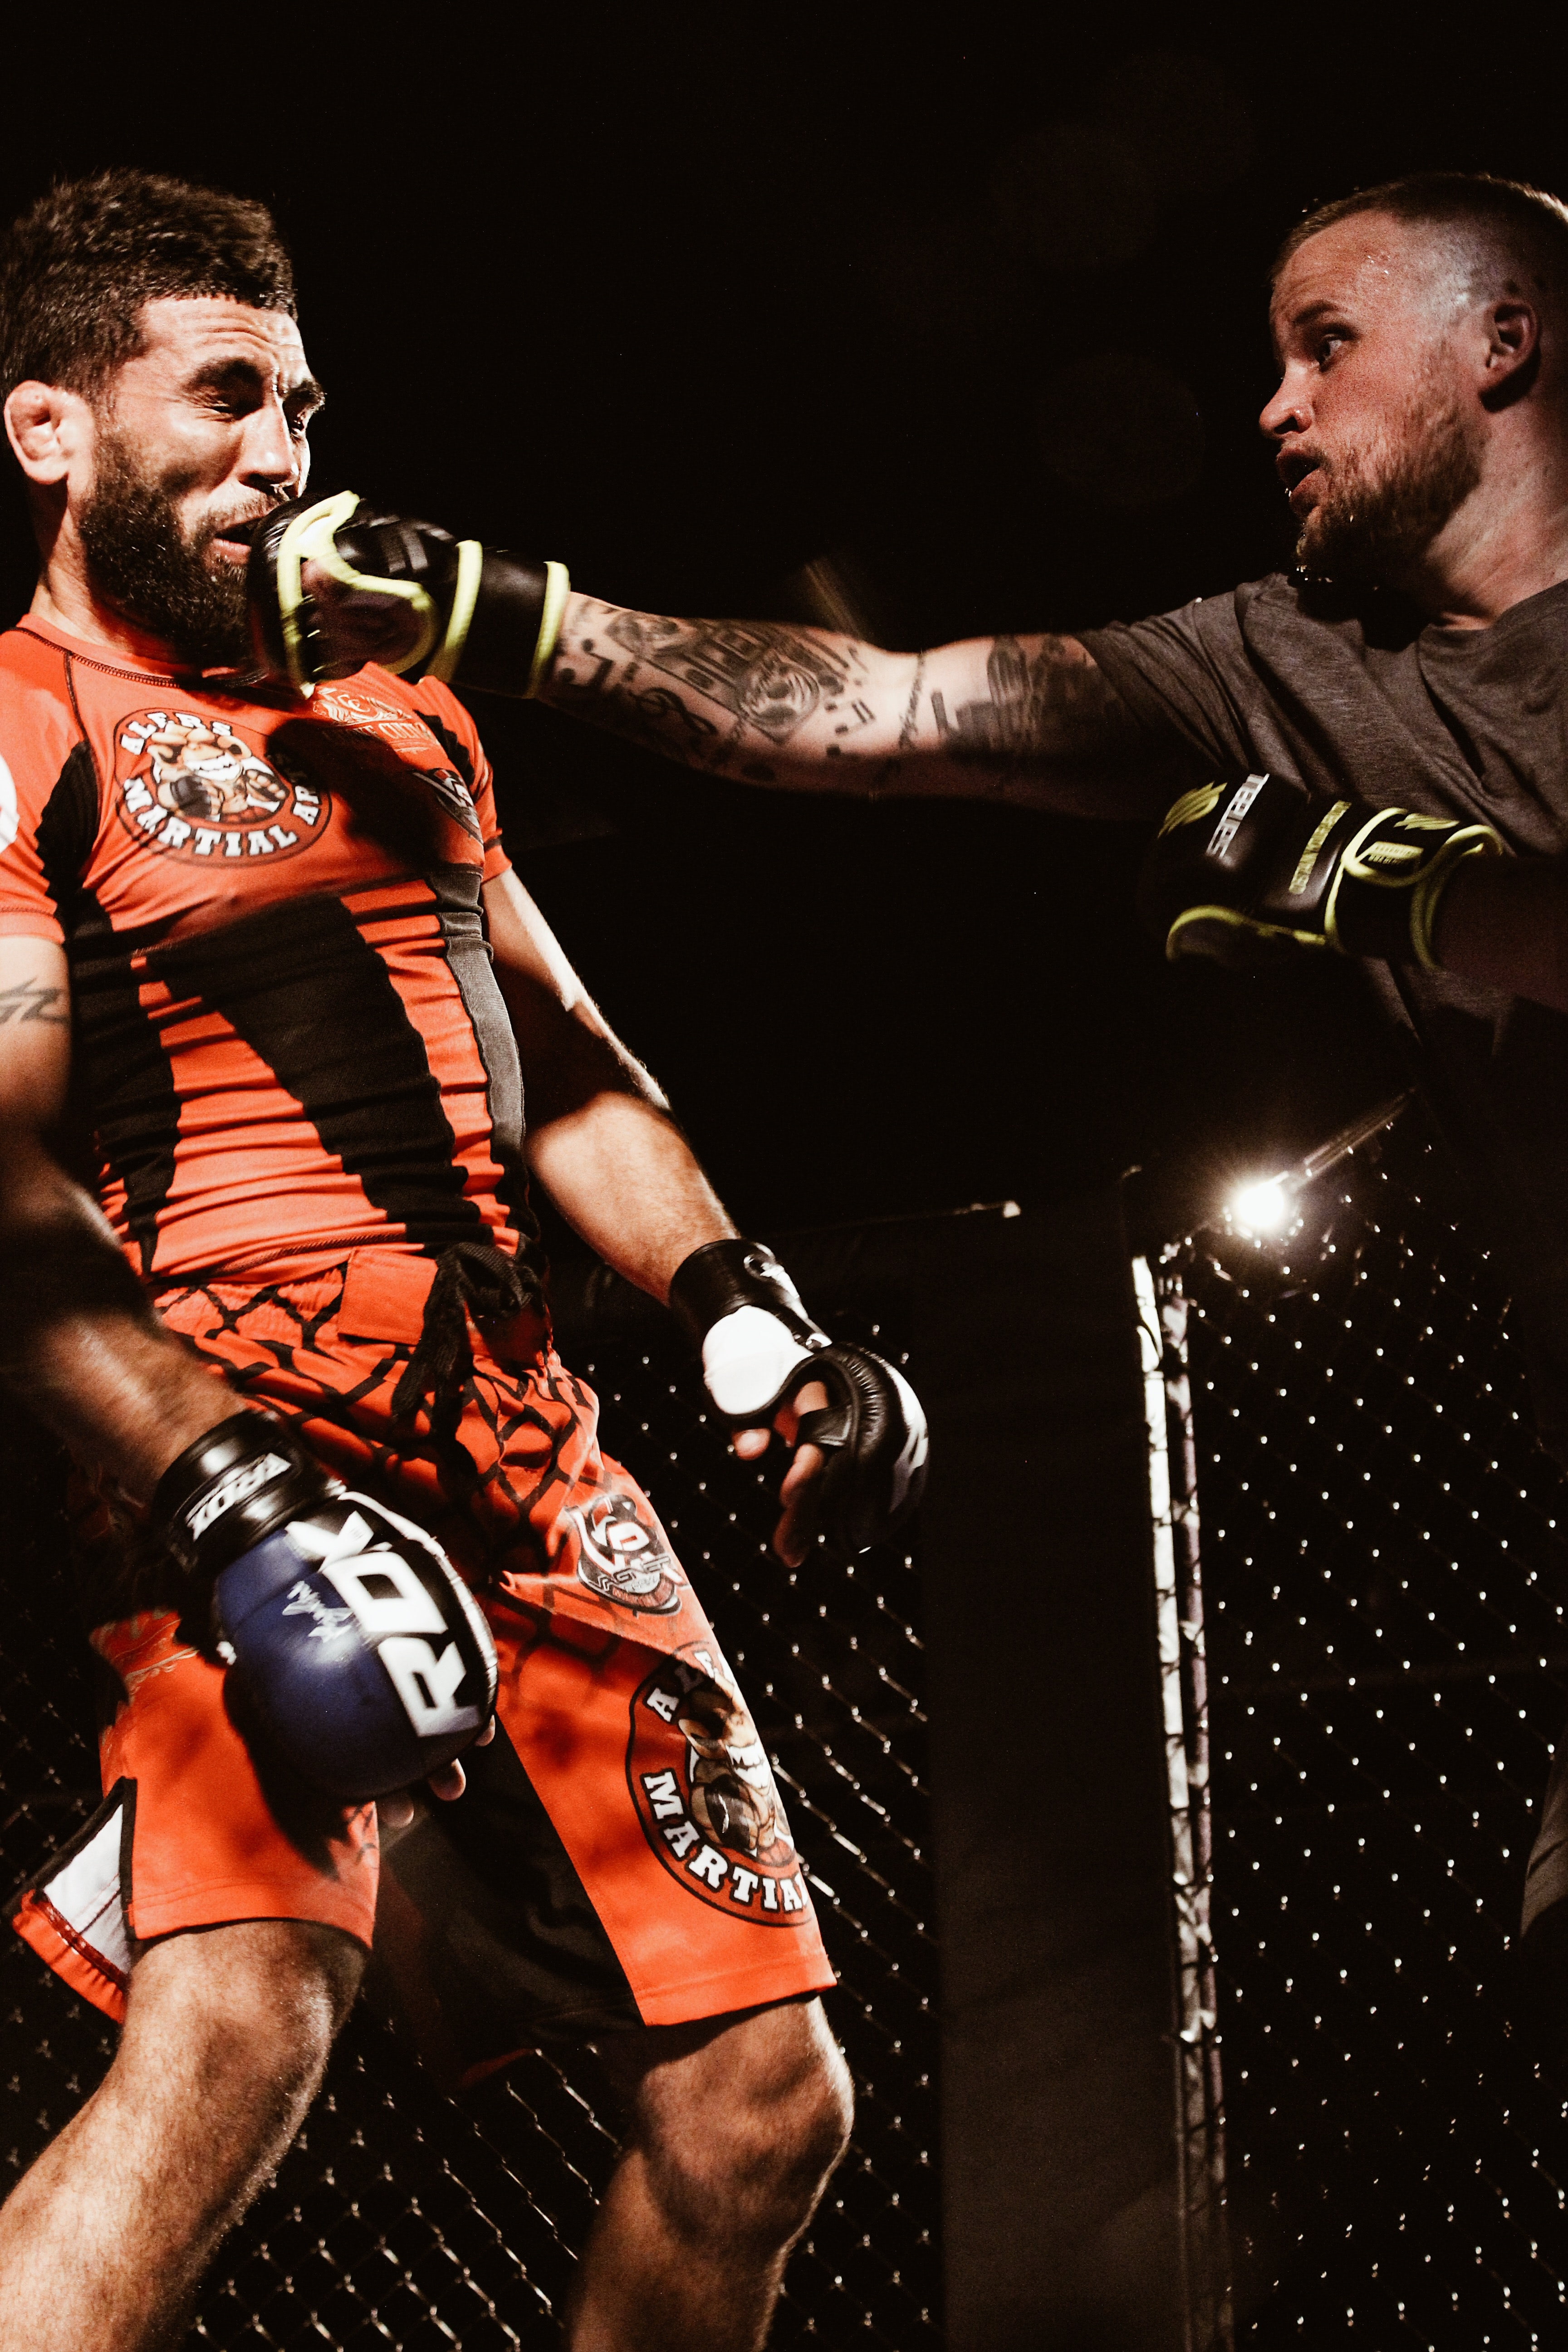
\includegraphics[width=0.6\textwidth]{boxer.jpg}
\end{center}
    
    \end{column}

    
    \end{columns}
    
\end{frame}



%% Arbeit, Energie, Leistng
 
 
 %% Eishockey, Frage 446
\begin{frame}{IMPP-Fragen zu M01.2}
    
    \textbf{
    Ein Eishockeypuck mit einer Masse von \(0,16\,kg\) wird bei einem Schlagschuss auf eine Geschwindigkeit von etwak \(180\,km/h\) (\(=50\, m/s\)) beschleunigt. (Zur Vereinfachung wird bei der Betrachtung von Geschwindigkeit und Energie des Pucks nur dessen Translations- und nicht auch eine Rotationsbewegung berücksichtigt).
    } 
    
    \textbf{
    Wie groß ist ungefähr die kinetische Energie des Pucks, wenn er aus kurzer Distanz - näherungsweise ohne jegliche vorherige Reibungsverluste - auf den Körper des Torwarts trifft?
    }\\[0.2 cm]

\begin{description}
\item{A.} \(40\,J\)
\item{B.} \(200\,J\) %% correct 
\item{C.} \(400\,J\)
\item{D.} \(800\,J\)
\item{E.} \(2\,kJ\)

\end{description}
    
    
\end{frame}


\begin{frame}{IMPP-Fragen zu M01.2}
    
    \textbf{
    Ein Eishockeypuck mit einer Masse von \(0,16\,kg\) wird bei einem Schlagschuss auf eine Geschwindigkeit von etwak \(180\,km/h\) (\(=50\, m/s\)) beschleunigt.  Wie groß ist ungefähr die kinetische Energie des Pucks, wenn er aus kurzer Distanz auf den Körper des Torwarts trifft?
    }\\[0.2 cm]

Kinetische Energie:  

\[
E = \frac{1}{2} m v^2 = 
\]

\pause

\[
\frac{1}{2} \times 0.16\,kg \times  50^2 \,\frac{m^2}{s^2} = 0.08 \times 2500\, \frac{kg\,m^2}{s^2} = 200\, J
\]

\end{frame}



\begin{frame}{IMPP-Fragen zu M01.2}
    
    \textbf{
    Ein Eishockeypuck mit einer Masse von \(0,16\,kg\) wird bei einem Schlagschuss auf eine Geschwindigkeit von etwak \(180\,km/h\) (\(=50\, m/s\)) beschleunigt. (Zur Vereinfachung wird bei der Betrachtung von Geschwindigkeit und Energie des Pucks nur dessen Translations- und nicht auch eine Rotationsbewegung berücksichtigt).
    } 
    
    \textbf{
    Wie groß ist ungefähr die kinetische Energie des Pucks, wenn er aus kurzer Distanz - näherungsweise ohne jegliche vorherige Reibungsverluste - auf den Körper des Torwarts trifft?
    }\\[0.2 cm]

\begin{description}
\item{A.} \(40\,J\)
\item{B.} \textcolor{red}{\(200\,J\)}  %% correct 
\item{C.} \(400\,J\)
\item{D.} \(800\,J\)
\item{E.} \(2\,kJ\)

\end{description}
    
    
\end{frame}




% %% Drehmoment, Trägheitsmoment, Drehimpuls
 
\begin{frame}{IMPP-Fragen zu M01.2}

    \textbf{
    Für die Bewegungsabläufe bei bestimmten Sportarten wie z.B. Eiskunstlauf, Turmspringen und Reckturnen ist der Satz von der Erhaltung des Drehimpulses bedeutsam.}
    
    \textbf{Durch welche der Aussagen lässt sich die Definition des Drehimpulses L am ehesten in Worte fassen?
    } \\[0.2 cm]
    
    \begin{description}
\item{A.} L ist das Produkt aus Geschwindigkeit und Masse
\item{B.} L ist das Produkt aus Masse und Beschleunigung
\item{C.} L ist das Produkt aus Trägheitsmoment und Winkelgeschwindigkeit %% correct
\item{D.} L ist der Quotient aus Masse und Winkelgeschwindigkeit
\item{E.}  L ist der Quotient aus Trägheitsmoment und Winkelgeschwindigkeit

\end{description}
    
\end{frame}


{ \usebackgroundtemplate{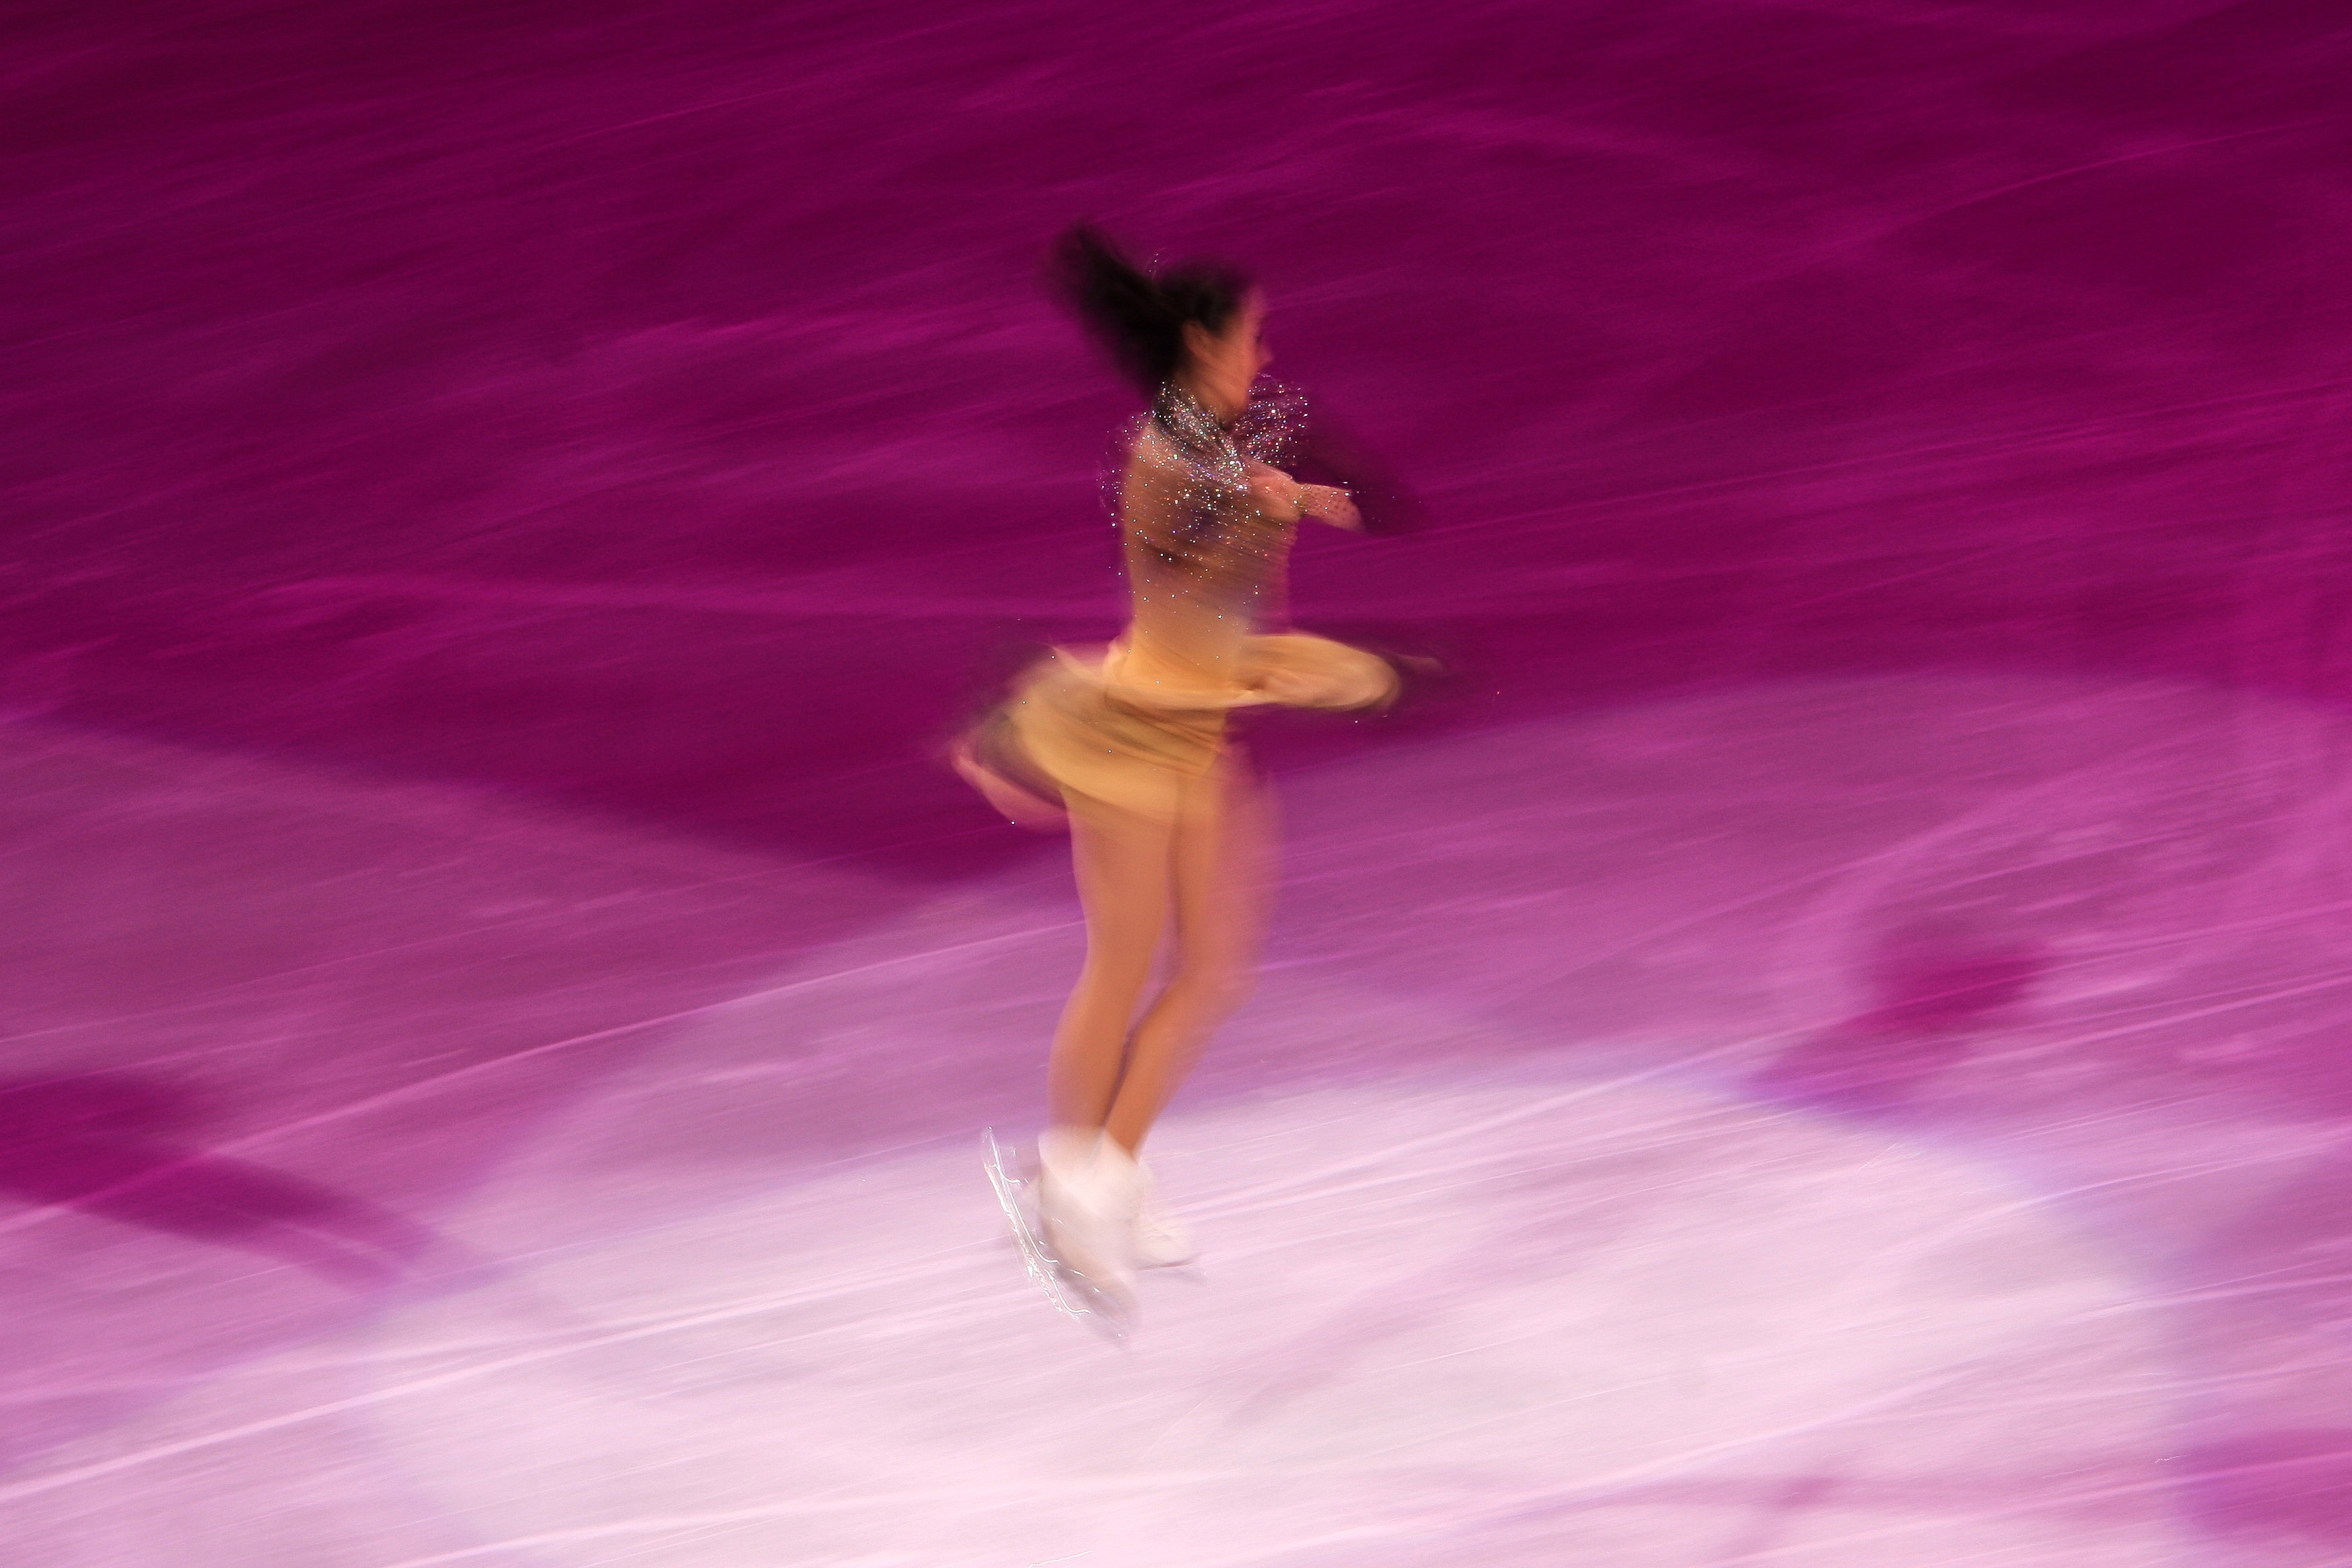
\includegraphics[width=1.2\paperwidth]{pirouette.jpg}} 
\begin{frame}{IMPP-Fragen zu M01.2}

\textcolor{white}{Wir erinnern uns}  \\ [6cm]


\end{frame}
}





\begin{frame}{IMPP-Fragen zu M01.2}

Es geht nicht um Masse allein, sondern wie sie verteilt ist. Mehr Masse weiter Weg vom Köper: größeres Trägheitsmoment.

\pause 

\begin{description}
\item{A.} \sout{L ist das Produkt aus Geschwindigkeit und Masse}
\item{B.} \sout{L ist das Produkt aus Masse und Beschleunigung}
\item{C.} L ist das Produkt aus Trägheitsmoment und Winkelgeschwindigkeit %% correct
\item{D.} \sout{L ist der Quotient aus Masse und Winkelgeschwindigkeit}
\item{E.}  L ist der Quotient aus Trägheitsmoment und Winkelgeschwindigkeit
\end{description}

\end{frame}




\begin{frame}{IMPP-Fragen zu M01.2}

Drehimpuls bleibt erhalten: Höhere Winkelgeschwindigkeit bei kleinerem Trägheitsmoment

\pause

\begin{description}
\item{A.} \sout{L ist das Produkt aus Geschwindigkeit und Masse}
\item{B.} \sout{L ist das Produkt aus Masse und Beschleunigung}
\item{C.} \textcolor{theme}{\textbf{L ist das Produkt aus Trägheitsmoment und Winkelgeschwindigkeit}} %% correct
\item{D.} \sout{L ist der Quotient aus Masse und Winkelgeschwindigkeit}
\item{E.}  \sout{L ist der Quotient aus Trägheitsmoment und Winkelgeschwindigkeit}
\end{description}

\end{frame}
    


   



\section{M01.3 Aerodynamik Hydrodynamik, Viskosität und Grenzflächeneffekte}

%% Learning Objectives


% Eigenschaften von Flüssigkeiten und Gasen erklären
% Druck definieren, Stempeldruck erklären
% Luftdruck erklären 
% Schweredruck in Flüssigkeiten und Auftrieb erklären
% Auswirkungen von Druck auf den menschlichen Organismus erklären
% Volumenstrom, Strömungswiderstand, Strömungsleitwert definieren 
% Kontinuitätsgleichung kennen 
% Kohäsion und Adhäsion definieren
% Den Kapillareffekt erklären und Beispiele gebeben
% Oberflächenspannung definieren

% Druck und Auftrieb berechnen
% Luftdruck an verschiedenen Orten abschätzen
% Schweredruck im Wasser abschätzen
% Volumenstrom, Strömungswiderstand, Strömungsleitwert berechnen
% Die Kontinuitätsgleichung anwenden
% Strömungsfelder durch Stromlinien darstellen
% Prinzipien der Strömung im Blutkreislauf und in der Atmung erkennen
% Den Bernoulli-Effekt mit Alltagsgegenständen demonstrieren
% Die Kirchhoff-Gesetze anwenden
% Das Hagen-Poiseuille Gesetz anwenden
% Erklären, warum Händewaschen in einer viralen Pandemie wichtig ist
% Die eigene Intuition im Hinblick auf Flüssigkeiten und Gase hinterfragen
% Die Augen offen halten für hydrodynamische und aerodynamische Effekte im Alltag und in der Medizin


%% Slides: 

% Druck
\begin{frame}{Druck}


\begin{columns}[c]



\begin{column}{5cm}

Druck = \(\frac{\text{Kraft}}{\text{Fläche}}\)


\begin{block}{Flüssigkeiten}

Flüssigkeiten sind nicht kompressibel. Deshalb: 
\begin{itemize}
    \item 
    können sie durch Druck bewegt werden
    \item
    ist Wasser unabhängig von der Tiefe überall gleich dicht
\end{itemize}

Schweredruck im Wasser: Höhe der Wassersäule \(\times\) Dichte \(\times\) Fallbeschleunigung 
\end{block}

\end{column}
\pause
\begin{column}{5cm}
\begin{block}{Gase}

Gase sind kompressibel, daher wird die Luft mit zunehmender Höhe dünner. \\

Faustregel für Luftdruck: Abnahme um \(1\,\%\) alle \SI{80}{\meter} oder \(10\,\%\) alle \SI{840}{\meter} \\[0.5 cm]

\end{block}

\begin{center}
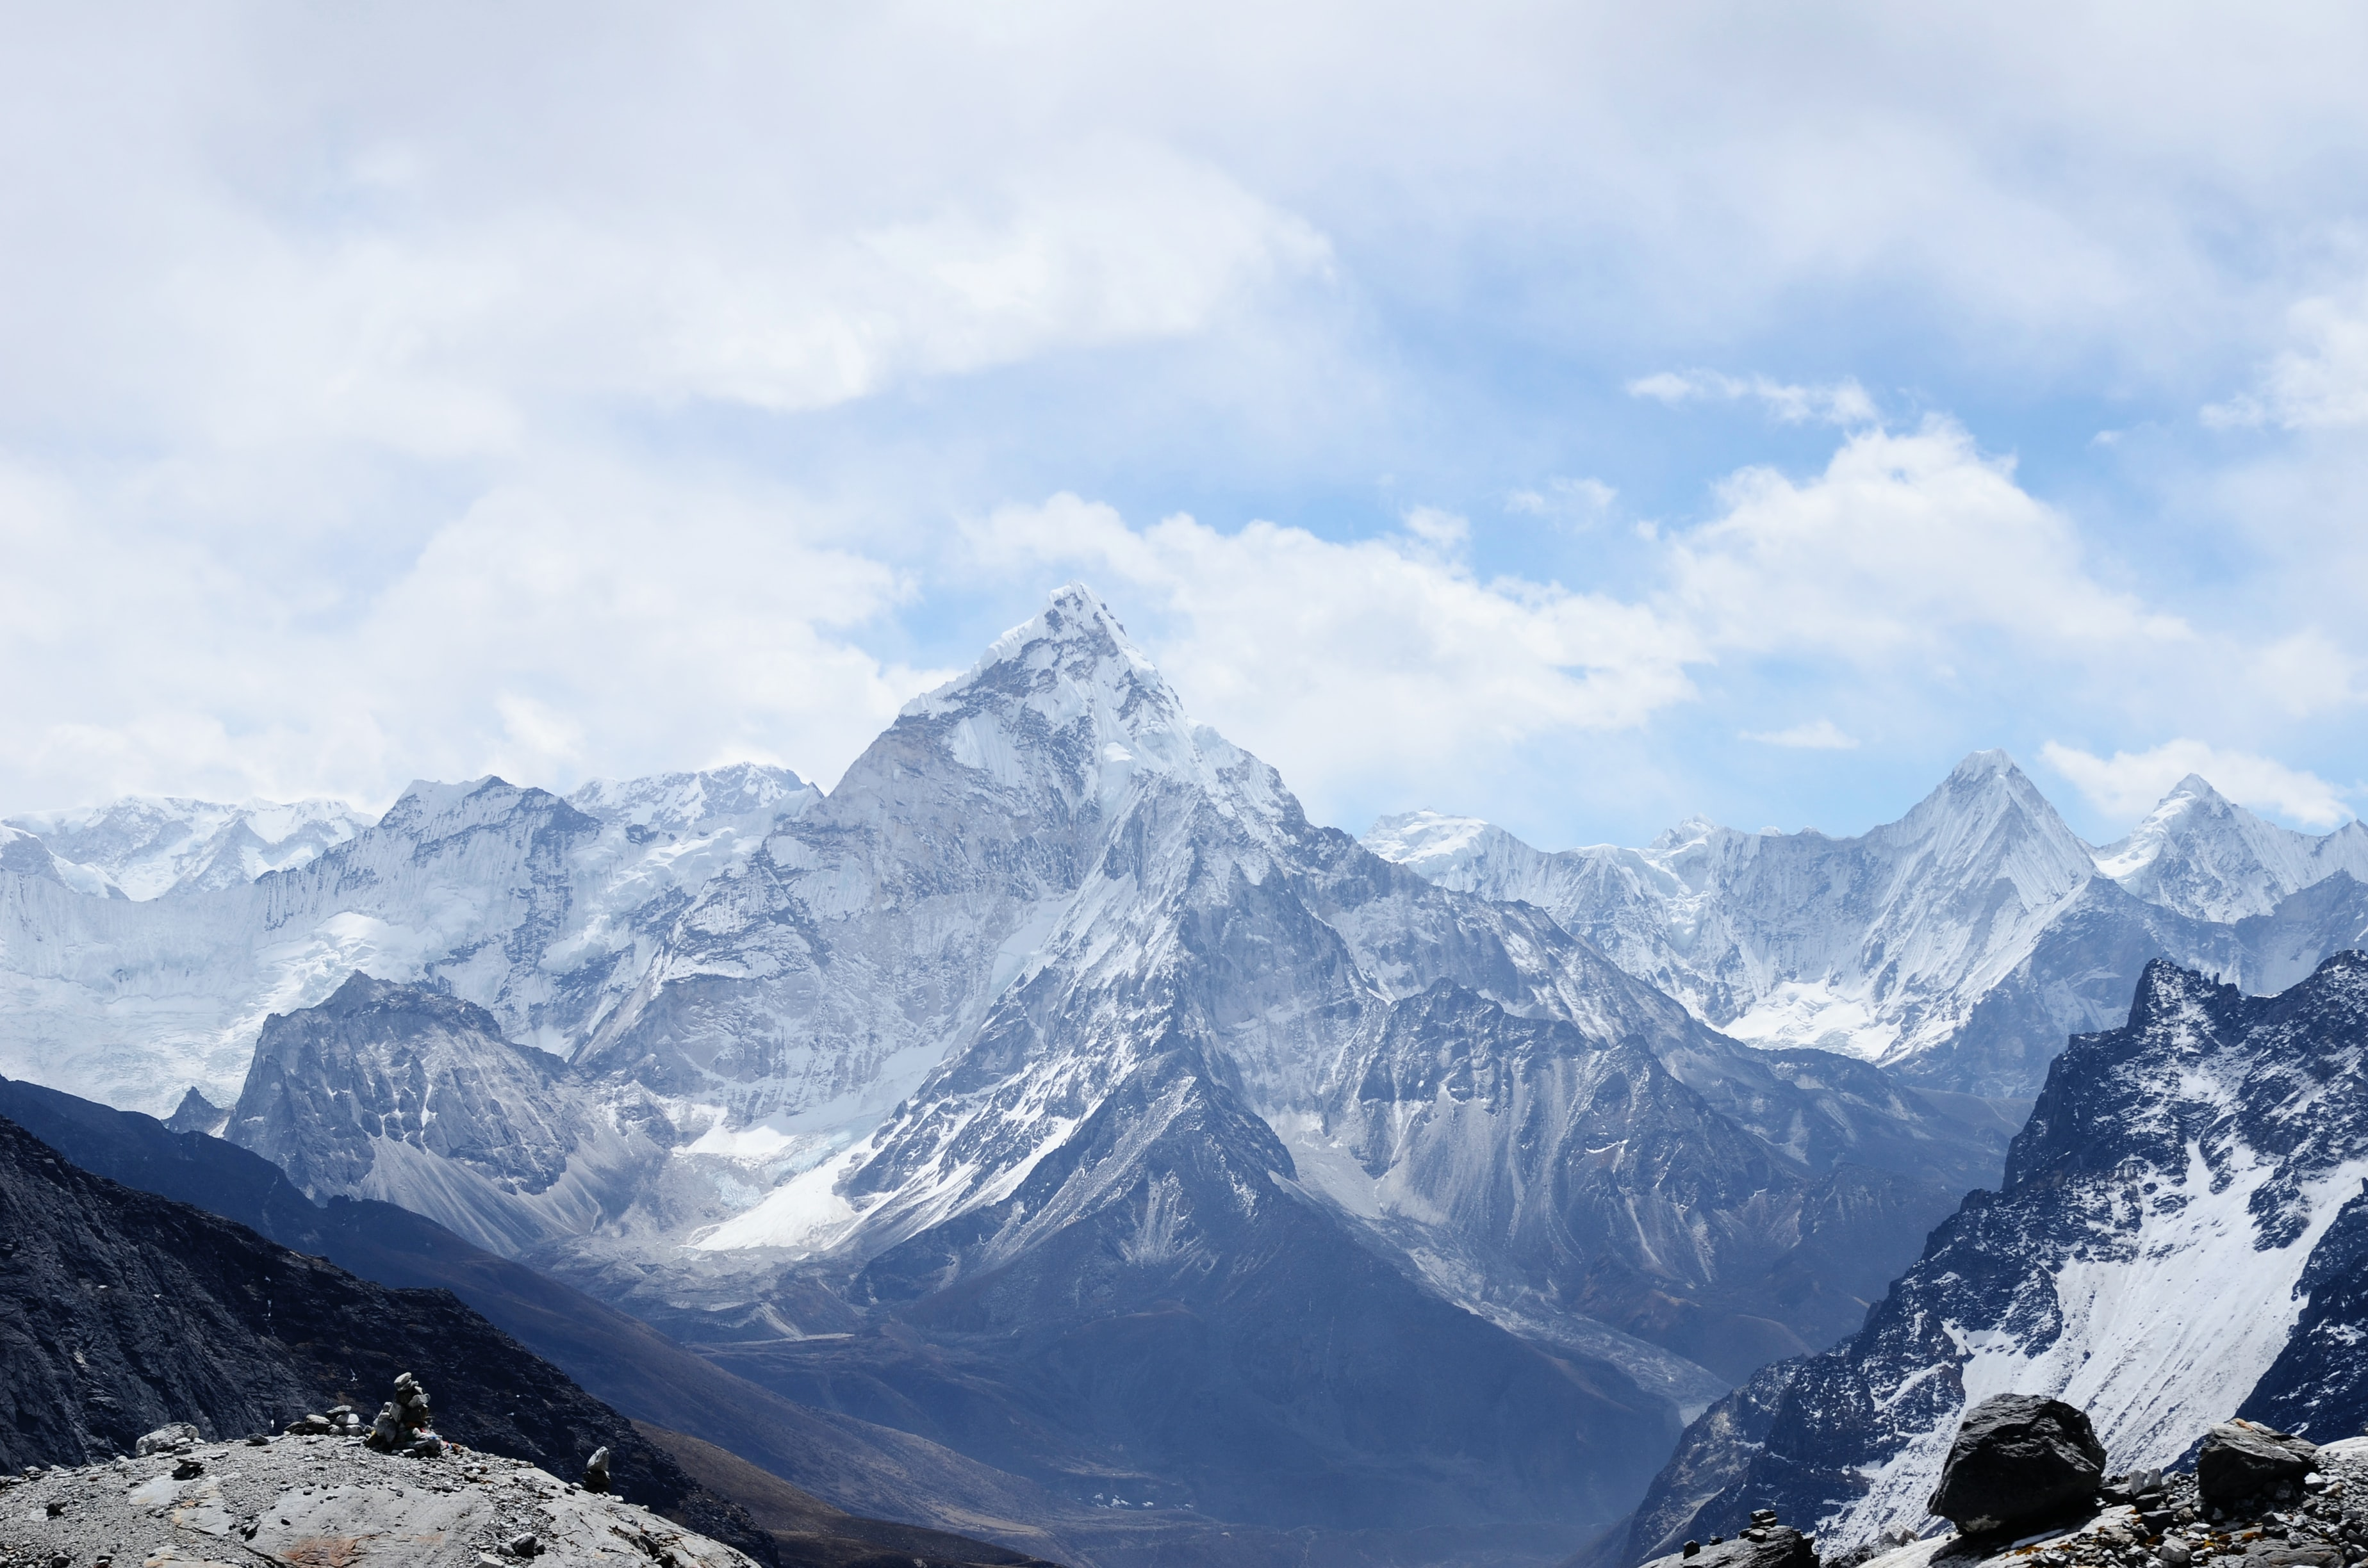
\includegraphics[width=\textwidth]{berge.jpg}    
\end{center}


\end{column}



\end{columns}

    
    
\end{frame}


% Strömung 
\begin{frame}{Strömung}
    Volumenstrom: Strömungsgeschwindigkeit \(\times\) Querschnittsfläche \\[0.2 cm]
    \pause
    Kontinuitätsgleichung: Volumenstrom bleibt konstant  \\
    (Kleinere Blutgefäße: Blut fließt schneller) \\[0.2 cm]
    \pause
    Bernoulli-Gesetz:  Höhere Strömungsgeschwindigkeit heißt niedrigerer Druck  \\
    (Kleinere Blutgefäße: Niedrigerer Druck) \\[0.2 cm]
    \pause
    Hagen-Poiseuille-Gesetz: 
 
    \[I=\frac{r^4\pi}{8\eta}\frac{\Delta p}{\Delta l}\]
 
    Volumenstrom größer, je größer Radius und Druck \\
    Volumenstrom größer, je kleiner Viskosität und Rohrlänge \\[0.2 cm]
    \pause
    Widerstand verhält sich analog zu elektrischem Strom
\end{frame}

% Kräfte an Grenzfläche


\begin{frame}{Kräfte an Grenzflächen}

\begin{block}{Kohäsion}

Zusammenhalt/Bindung zwischen Molekülen \textbf{desselben} Stoffes

\end{block}

\begin{block}{Adhäsion}

Zusammenhalt/Bindung zwischen Molekülen \textbf{verschiedener} Stoffe

\end{block}

Kapillareffekt als Folge der Adhäsion \\[0.5 cm]

\pause

\begin{columns}[c]
\begin{column}{5cm}
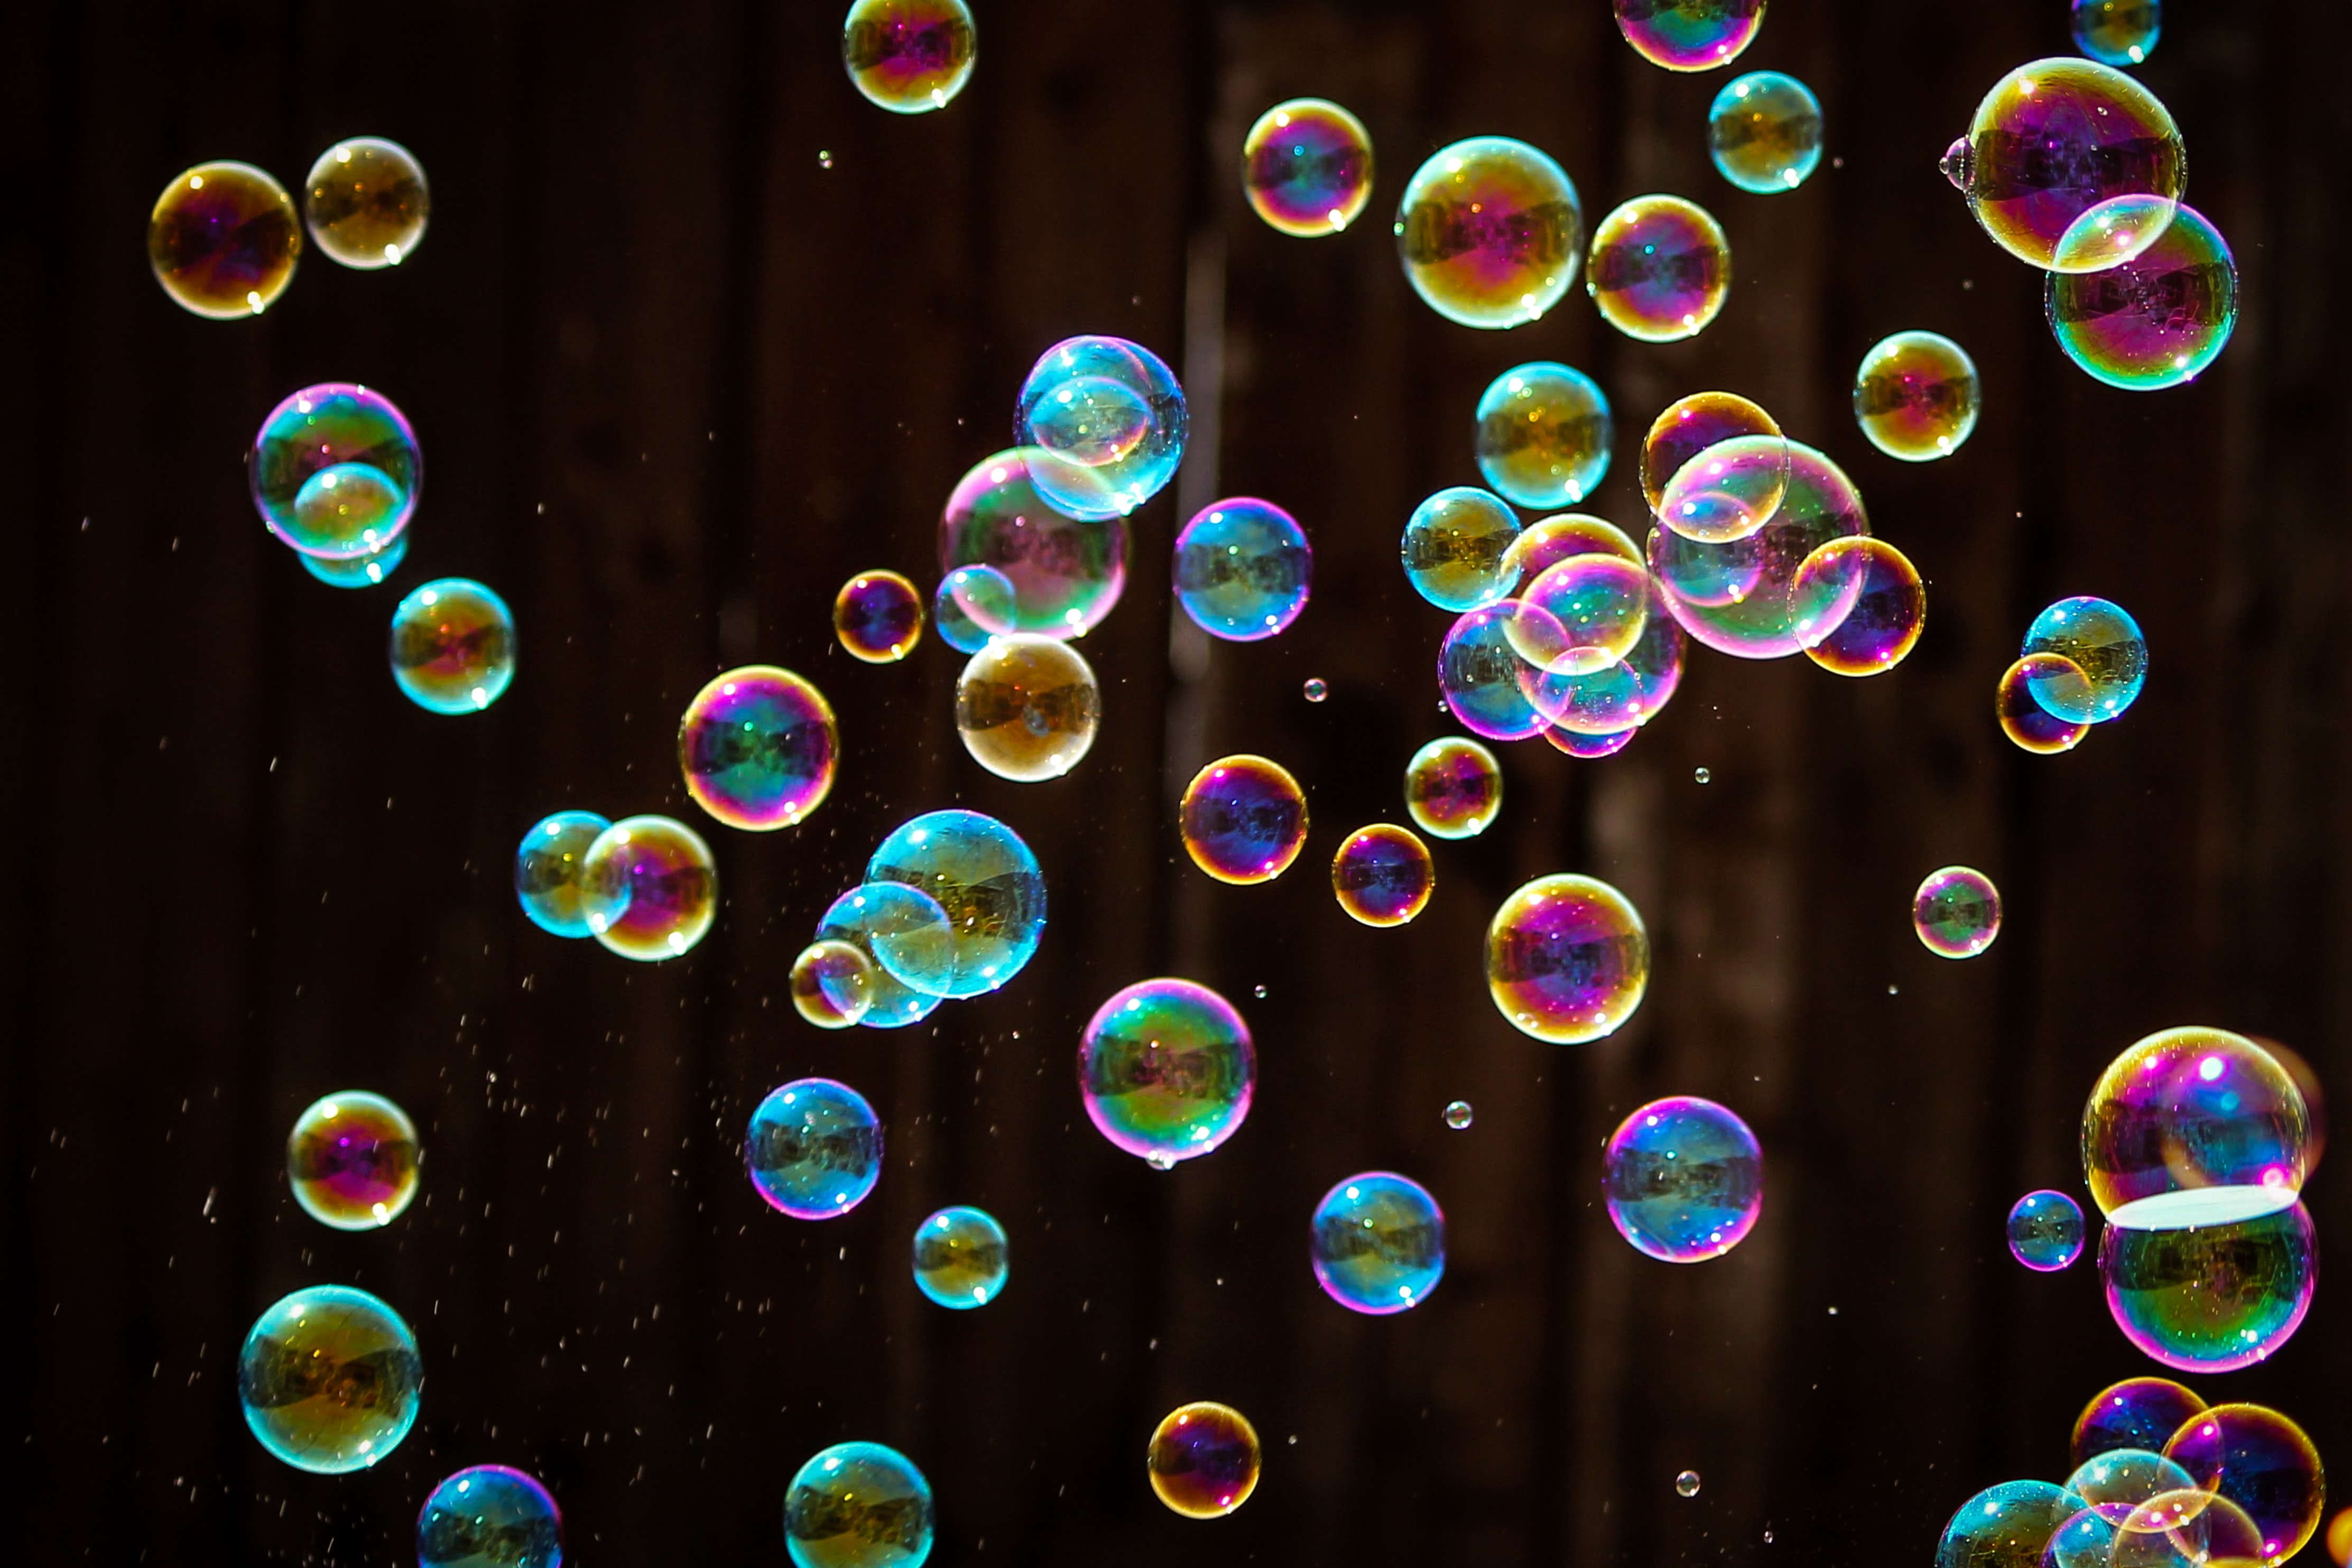
\includegraphics[width=\textwidth]{seifenblasen.jpg}
\end{column}

\begin{column}{5cm}
Oberflächenspannung = $\frac{\text{Oberflächenenergie}}{\text{Oberfläche}}$ \\[0.5 cm]

Flüssigkeiten wollen ihre Oberfläche minimieren


\end{column}


\end{columns}

    
\end{frame}

%% Druck
\begin{frame}{IMPP-Fragen zu M01.3}
    \textbf{Bei einem Patienten wird eine hyperbare Sauerstofftherapie durchgeführt, wobei sich in der Druckkammer als Gas nahezu reiner Sauerstof bei einem Kammerdruck von \(2\,500\,hPa\) befindet. 
        } \\
        \textbf{
        Etwa wievielfach höher ist dieser (Sauerstoffpartial-)Druck als der Sauerstoffpartialdruck von normaler Luft unter normalem Luftdruck
        }\\[0.2 cm]

\begin{description}
\item{A.} 2-fach
\item{B.} 5-fach
\item{C.} 8-fach
\item{D.} 12-fach %% correct
\item{E.} 20-fach

\end{description}
\end{frame}


\begin{frame}{IMPP-Fragen zu M01.3}
    \textbf{Bei einem Patienten wird eine hyperbare Sauerstofftherapie durchgeführt, wobei sich in der Druckkammer als Gas nahezu reiner Sauerstoff bei einem Kammerdruck von \(2\,500\,hPa\) befindet. 
        } \\
        \textbf{
        Etwa wievielfach höher ist dieser (Sauerstoffpartial-)Druck als der Sauerstoffpartialdruck von normaler Luft unter normalem Luftdruck?
        }\\[0.2 cm]

2 Sachen müssen wir wissen: \\
1. Wieviel höher ist der Lufdruck in der Kammer als normal? \\
2. Wieviel größer ist der Sauerstoffanteil als in normaler Luft? \\



\end{frame}


\begin{frame}{IMPP-Fragen zu M01.3}
    \textbf{Bei einem Patienten wird eine hyperbare Sauerstofftherapie durchgeführt, wobei sich in der Druckkammer als Gas nahezu reiner Sauerstoff bei einem Kammerdruck von \(2\,500\,hPa\) befindet. 
        } \\
        \textbf{
        Etwa wievielfach höher ist dieser (Sauerstoffpartial-)Druck als der Sauerstoffpartialdruck von normaler Luft unter normalem Luftdruck?
        }\\[0.2 cm]

2 Sachen müssen wir wissen: \\
1. Wieviel höher ist der Lufdruck in der Kammer als normal? \\ \pause

Normaler Lufdruck (in Seehöhe) ist rund \(1\,000\,hPa\), \\ Kammer daher \(2.5\times\) höher.

\pause

2. Wieviel größer ist der Sauerstoffanteil als in normaler Luft? \\

Sauerstoffanteil in normaler Luft: \(21\,\%\), in Kammer fast \(100\,\%\), \\ 
also ca. \(5\times\) höher \pause

\[2.5\times 5 \approx 12.5\]

\end{frame}


\begin{frame}{IMPP-Fragen zu M01.3}
    \textbf{Bei einem Patienten wird eine hyperbare Sauerstofftherapie durchgeführt, wobei sich in der Druckkammer als Gas nahezu reiner Sauerstof bei einem Kammerdruck von \(2\,500\,hPa\) befindet. 
        } \\
        \textbf{
        Etwa wievielfach höher ist dieser (Sauerstoffpartial-)Druck als der Sauerstoffpartialdruck von normaler Luft unter normalem Luftdruck?
        }\\[0.2 cm]

\begin{description}
\item{A.} 2-fach
\item{B.} 5-fach
\item{C.} 8-fach
\item{D.} \textcolor{theme}{\textbf{12-fach}} %% correct
\item{E.} 20-fach

\end{description}
\end{frame}


%% Strömung

\begin{frame}{IMPP-Fragen zu M01.3}


    \textbf{
    Für den Strömungswiderstand R einer Arteriole gilt in Abhängigkeit von deren Länge l und Radios r sowie der Viskosität \(\eta\) der hindurchströmenden Flüssigkeit (wobei vereinfachend das Hagen-Poiseuille-Gesetz als gültig angenommen wird):
    } \\[0.2 cm]

\begin{description}
\item{A.}
\(R=\frac{8\cdot l\cdot \eta}{\pi \cdot r^2}\)
\item{B.}
\(R=\frac{8\cdot l\cdot \eta}{\pi \cdot r^4}\)  %% correct
\item{C.}
\(R=\frac{8\cdot l}{\eta \cdot \pi  \cdot r^4}\)
\item{D.}
\(R=\frac{\pi \cdot r^2}{8\cdot l \cdot \eta}\)
\item{E.}
\(R=\frac{\pi\cdot r^4}{8\cdot l \cdot \eta}\)
\end{description}
\end{frame}


\begin{frame}{IMPP-Fragen zu M01.3}

Idealerweise können wir Hagen-Poiseuille und wissen, dass der Widerstand umgekehrt proportional zum Volumenstrom ist. \\

\pause
Aber selbst wenn nicht: \pause \\
 
Würde der Widerstand mit der Rohr-Querschnittsfläche \(r^2 \pi\) zu- oder abnehmen?

\end{frame}

\begin{frame}{IMPP-Fragen zu M01.3}

\begin{description}
\item{A.}
\(R=\frac{8\cdot l\cdot \eta}{\pi \cdot r^2}\)
\item{B.}
\(R=\frac{8\cdot l\cdot \eta}{\pi \cdot r^4}\)  %% correct
\item{C.}
\(R=\frac{8\cdot l}{\eta \cdot \pi  \cdot r^4}\)
\item{D.}
\sout{\(R=\frac{\pi \cdot r^2}{8\cdot l \cdot \eta}\)}
\item{E.}
\sout{\(R=\frac{\pi\cdot r^4}{8\cdot l \cdot \eta}\)}
\end{description}
\end{frame}

\begin{frame}{IMPP-Fragen zu M01.3}

Idealerweise können wir Hagen-Poiseuille und wissen, dass der Widerstand umgekehrt proportional zum Volumenstrom ist. \\

Aber selbst wenn nicht:  \\
  
Würde der Widerstand mit der Rohr-Querschnittsfläche \(r^2 \pi\) zu- oder abnehmen? \\
Würde der Widerstand mit der Viskosität \(\eta\) zu- oder abnehmen? 

\end{frame}

\begin{frame}{IMPP-Fragen zu M01.3}

\begin{description}
\item{A.}
\(R=\frac{8\cdot l\cdot \eta}{\pi \cdot r^2}\)
\item{B.}
\(R=\frac{8\cdot l\cdot \eta}{\pi \cdot r^4}\)  %% correct
\item{C.}
\sout{\(R=\frac{8\cdot l}{\eta \cdot \pi  \cdot r^4}\)}
\item{D.}
\sout{\(R=\frac{\pi \cdot r^2}{8\cdot l \cdot \eta}\)}
\item{E.}
\sout{\(R=\frac{\pi\cdot r^4}{8\cdot l \cdot \eta}\)} \\[0.2 cm]
\end{description}


\pause
Dann haben wir eine 50:50 Chance, und müssen uns nur noch daran errinern, dass beim Hagen-Poiseuille-Gesetz "irgendwas mit \(r^4\)" war

\end{frame}


\begin{frame}{IMPP-Fragen zu M01.3}


    \textbf{
    Für den Strömungswiderstand R einer Arteriole gilt in Abhängigkeit von deren Länge l und Radios r sowie der Viskosität \(\eta\) der hindurchströmenden Flüssigkeit (wobei vereinfachend das Hagen-Poiseuille-Gesetz als gültig angenommen wird):
    } \\[0.2 cm]

\begin{description}
\item{A.}
\sout{\(R=\frac{8\cdot l\cdot \eta}{\pi \cdot r^2}\)}
\item{B.}
\textcolor{theme}{\(R=\frac{8\cdot l\cdot \eta}{\pi \cdot r^4}\) } %% correct
\item{C.}
\sout{\(R=\frac{8\cdot l}{\eta \cdot \pi  \cdot r^4}\)}
\item{D.}
\sout{\(R=\frac{\pi \cdot r^2}{8\cdot l \cdot \eta}\)}
\item{E.}
\sout{\(R=\frac{\pi\cdot r^4}{8\cdot l \cdot \eta}\)}
\end{description}
\end{frame}




%% Mehr Strömung, denn zu Kräften an Grenzflächen gibt es quasi keine IMPP Fragen


\begin{frame}{IMPP-Fragen zu M01.3}
    \textbf{In einer Aorta strömt bei einer Innenquerschnittsfläche von etwa \(4\,cm^2\) Blut mit einer mittleren Geschwindigkeit von etwa \(20\,cm/s\). Die nachgeschalteten Blutgefäße verzweigen sich in die zugehörigen Kapillaren. Die Gesamtquerschnittsfläche (Summe der Innenquerschnittsflächen) dieser Kapillaren beträgt etwa \(3\,000\,cm^2\)}
    
    \textbf{
    Etwa wie groß ist somit die mittlere Strömungsgeschwindigkeit in den Kapillaren?
    }\\[0.2 cm]

\begin{description}
\item{A.} \(0,03\,cm/s\)
\item{B.} \(0,09\,cm/s\)
\item{C.} \(0,3\,cm/s\)
\item{D.} \(0,9\,cm/s\)
\item{E.} \(3\,cm/s\)

\end{description}
\end{frame}

\begin{frame}{IMPP-Fragen zu M01.3}
    \textbf{In einer Aorta strömt bei einer Innenquerschnittsfläche von etwa \(4\,cm^2\) Blut mit einer mittleren Geschwindigkeit von etwa \(20\,cm/s\). Die nachgeschalteten Blutgefäße verzweigen sich in die zugehörigen Kapillaren. Die Gesamtquerschnittsfläche (Summe der Innenquerschnittsflächen) dieser Kapillaren beträgt etwa \(3\,000\,cm^2\)}
    
    \textbf{
    Etwa wie groß ist somit die mittlere Strömungsgeschwindigkeit in den Kapillaren?
    }\\[0.2 cm]

\begin{columns}[c]

\begin{column}{3cm}

%% pictures: Aorta, Kapillaren
\begin{center}
    \includegraphics<1>[width=\textwidth]{kapillaren_parallel.jpeg}
    \includegraphics<2->[width=\textwidth]{kapillaren_eins.jpeg}

\end{center}
 \end{column}

\begin{column}{7cm}


Parallelschaltung: Stromflüsse können einfach addiert werden; der Gesamtfluss verhält sich so, als hätten wir ein einzelnes nachgeschaltetes Blutgefäß mit \(3\,000\,cm^2\). \\[0.2 cm]

\pause
\pause

Kontinuitätsgleichung: \(v_1\,A_1=v_2\,A_2\)

\[v = \frac{4\,cm^2 \times 20\,cm/s}{3\,000\,cm^2} \approx 0.03\,cm/s\]


\end{column}


\end{columns}

\end{frame}







\begin{frame}{IMPP-Fragen zu M01.3}
    \textbf{In einer Aorta strömt bei einer Innenquerschnittsfläche von etwa \(4\,cm^2\) Blut mit einer mittleren Geschwindigkeit von etwa \(20\,cm/s\). Die nachgeschalteten Blutgefäße verzweigen sich in die zugehörigen Kapillaren. Die Gesamtquerschnittsfläche (Summe der Innenquerschnittsflächen) dieser Kapillaren beträgt etwa \(3\,000\,cm^2\)}
    
    \textbf{
    Etwa wie groß ist somit die mittlere Strömungsgeschwindigkeit in den Kapillaren?
    }\\[0.2 cm]

\begin{description}
\item{A.} \textcolor{red}{\(0,03\,cm/s\)}
\item{B.} \(0,09\,cm/s\)
\item{C.} \(0,3\,cm/s\)
\item{D.} \(0,9\,cm/s\)
\item{E.} \(3\,cm/s\)

\end{description}
\end{frame}



\section{M01.5 Schwingungen und Wellen}



% \begin{block}{Wissen:}
% \begin{itemize}
% %%%%%
% \item
% Schwingungen und Wellen definieren
% \item
% Charakteristika von Schwingungen und Wellen benennen 
% \item
% Arten von Schwingungen und Wellen unterscheiden
% \item
% Erzwungene Schwingungen definieren und erklären
% \item
% Phänomene bei der Überlagerung von Wellen erklären
% \item
% Den Doppler-Effekt erklären
% \item
% Beispiele für den Doppler-Effekt geben
% \item
% Eigenschaften von Schallwellen benennen
% \item
% Eigenschaften elektromagnetischer Wellen benennen
% \item
% Unterschiede und Gemeinsamkeiten zwischen elektromagnetischen Wellen und Schallwellen angeben
% \item
% Das Konzept der Fourieranalyse erklären und Anwendungen nennen
% \end{itemize}

% \end{block}

% \end{frame}

% \begin{frame}

% \frametitle{Nach dieser Vorlesung sollten Sie:}
 

% \begin{block}{Können:}
% \begin{itemize}
% \item
% Charakteristika von Schwingungen und Wellen berechnen
% \item
% Graphische Darstellungen von Schwingungen und Wellen interpretieren
% \item
% Änderungen der Schallstärke berechnen
% \item
% Mit Klavieren experimentieren (und auch sonst) 
% \end{itemize}
% \end{block}

% \begin{block}{Fühlen:}

% \begin{itemize}
% \item
% Keine Angst vor Fouriertransformationen haben
% \item
% Schwingungen und Wellen im Alltag sehen 


% \end{itemize}

% \end{block}



%% Slides
%% Schwingungen
\begin{frame}{(Harmonische) Schwingungen}

\begin{center}

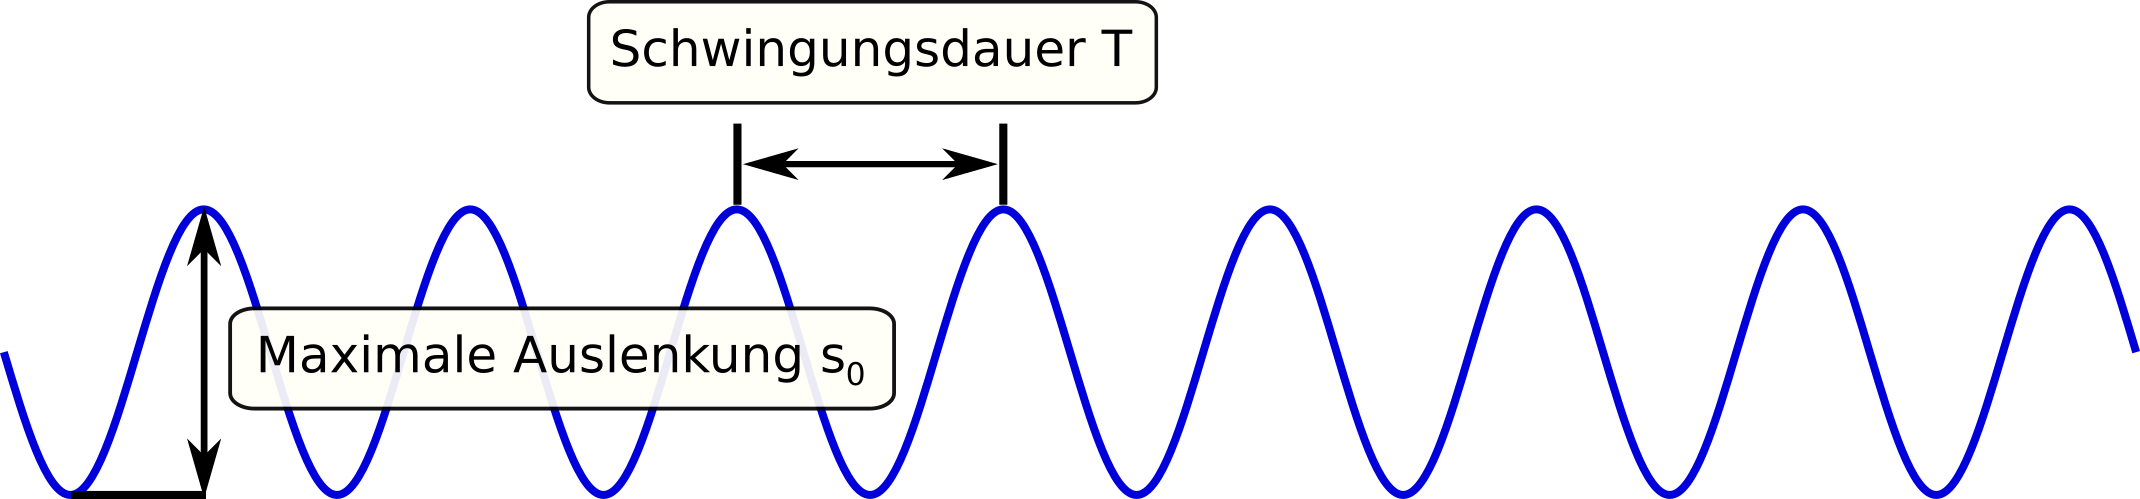
\includegraphics[width=0.8\textwidth]{schwingungen_groessen.png}
\end{center}


\begin{columns}[c]

\begin{column}{5cm}


\pause

Auslenkung \(s\) zum Zeitpunkt \(t\)

\[
s(t) = s_0\sin\frac{2\pi t}{T} =  \]
\[
s_0\sin (2\pi\nu t) = s_0 \sin (\omega t)
\]

$\,$\\[0.2 cm]

(bei Frequenz \(\nu = \frac{1}{T}\) und Kreisfrequenz \(\omega = 2\pi\nu\))

\end{column}

\begin{column}{5cm}

\pause
\begin{block}{Gedämpfte Schwingungen}

\[
s(t) = s_0 \sin (\omega t)  e^{-\delta t}
\]


\end{block}

\pause

\begin{block}{Erzwungene Schwingungen}

Bei Kopplung von zwei Schwingungen mit Frequenzen \(\nu_1\), \(\nu_2\). \\ Sind \(\nu_1\) und \(\nu_2\) Vielfache voneinander: Resonanz

\end{block}

\end{column}


\end{columns}


    
\end{frame}


%% Wellen

\begin{frame}{Wellen}
    Klassifikation nach Ausbreitungsrichtung: longitudinal vs transversal \\[0.2 cm]
    \pause
    Ausbreitungsgeschwindigkeit = Frequenz \(\times\) Wellenlänge \\
    Lichtgeschwindigkeit im Vakuum: \(300\,000\,000\,ms^{-1}\) \\
    Schallgeschwindigkeit in der Luft: \(330\,ms^{-1}\) \\
    Schallgeschwindigkeit im Wasser: \(1\,500\,ms^{-1}\) \\[0.2 cm]
\pause
Bei Überlagerung: Schwebung oder Interferenz \\[0.2 cm]
\pause
Doppler-Effekt: Gemessene Frequenz hängt von Bewegung relativ zur Quelle ab \\[0.2 cm]
\pause
Fourier-Analyse: Umrechnung vom Zeitbereich in den Frequenzbereich
\end{frame}



%% Schall und elektromagnetische Wellen
\begin{frame}{Schallwellen vs elektromagnetische Wellen}
    
\begin{tabular}{|l|l|l|}
\hline
        & \color{theme}{\textbf{Schallwellen}}  & \color{theme}{\textbf{Elektromagnetische Wellen}}     \\
\hline
Ausbreitung       & \SI{330}{\meter\per\second} (Luft)  &  \(\sim\)\SI{300\,000\,000}{\meter\per\second} (Vakuum)   \\
\hline
Richtung        & longitudinal  & transversal   \\
\hline
Medium          & nötig (z.B. Luft)        & nicht nötig \\ 
&                       & (können sich im Vakuum ausbreiten)       \\[0.2 cm]
\hline
\end{tabular}

\pause


\begin{columns}[c]

\begin{column}{6cm}

Schallintensität (physikalische Größe): \(\frac{W}{m^2}\)  \\
\pause
Schallstärke (relative Schallintensität, verglichen mit \(10^{-12} \,\frac{W}{m^2}\), logarithmische Skala): (Dezi-)Bel \\
\pause
Lautstärke (bezogen auf menschlichen Hörapparat, daher abhängig von Frequenz): Phon \\ 

\end{column}

\begin{column}{5cm}
      \begin{center}
          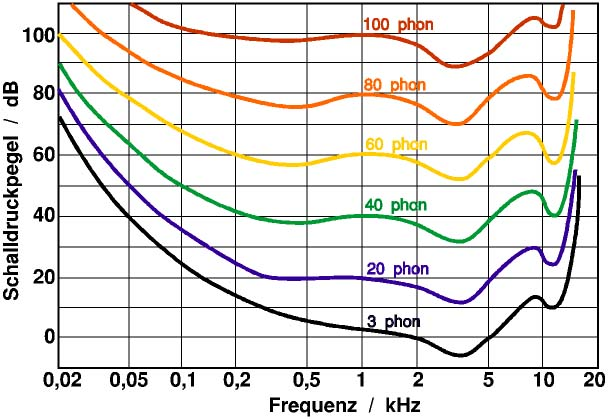
\includegraphics[width=\textwidth]{Akustik_db2phon.jpg}
      \end{center}

\end{column}

\end{columns}
      
      
\end{frame}




%% IMPP Fragen
%% Schwingungen
\begin{frame}{IMPP-Fragen zu M01.5}
    
    \textbf{In der Sonografie werden Schallwellen für bildgebende Verfahren eingesetzt. In Flüssigkeiten und Gasen breitet sich Schall als longitudinale Welle aus.}
    
    \textbf{
    Longitudinale Wellen ind am ehesten dadurch charakterisiert, dass 
    } \\[0.2 cm]

\begin{description}
\item{A.} ihre Schwingung in Richtung der Ausbreitungsrichtung erfolgt %% correct
\item{B.} sie ihre Schwingungsfrequenz ändern, wenn sie in ein Gewebe mit einer anderen Dichte übergehen
\item{C.} sie langwellige elektromagnetische Wellen sind
\item{D.} sie nur in einem Frequenzbereich von \(1\,MHz\) bis \(1\,THz\) auftreten
\item{E.} sie sich wie Licht durch Polarisatoren in unterschiedliche Schwingungsebenen polarisieren lassen

\end{description}
    
\end{frame}

\begin{frame}{IMPP-Fragen zu M01.5}
    
    

Wir erinnern uns: Longitudinale Wellen sind im Prinzip "Regenwurmwellen" 

\begin{center}
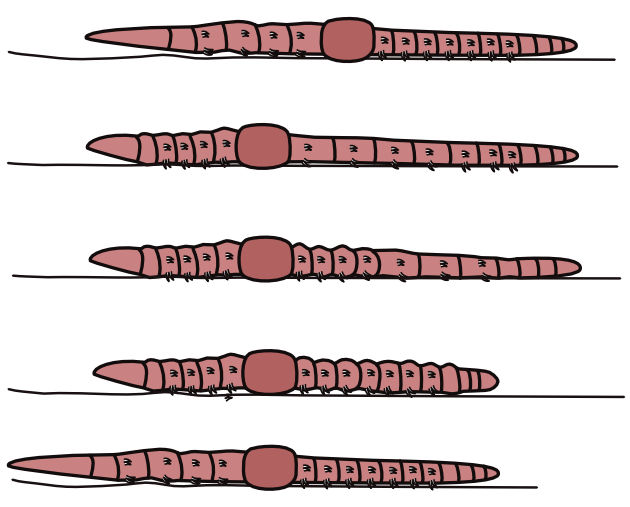
\includegraphics[width=0.6\textwidth]{regenwurm.png}
\end{center}






\end{frame}



\begin{frame}{IMPP-Fragen zu M01.5}
    
    \textbf{In der Sonografie werden Schallwellen für bildgebende Verfahren eingesetzt. In Flüssigkeiten und Gasen breitet sich Schall als longitudinale Welle aus.}
    
    \textbf{
    Longitudinale Wellen ind am ehesten dadurch charakterisiert, dass 
    } \\[0.2 cm]

\begin{description}
\item{A.} \textcolor{theme}{\textbf{ihre Schwingung in Richtung der Ausbreitungsrichtung erfolgt}}
\item{B.} sie ihre Schwingungsfrequenz ändern, wenn sie in ein Gewebe mit einer anderen Dichte übergehen
\item{C.} sie langwellige elektromagnetische Wellen sind
\item{D.} sie nur in einem Frequenzbereich von \(1\,MHz\) bis \(1\,THz\) auftreten
\item{E.} sie sich wie Licht durch Polarisatoren in unterschiedliche Schwingungsebenen polarisieren lassen

\end{description}
    
\end{frame}





 

%% Wellen

\begin{frame}{IMPP-Fragen zu M01.5}
\textbf{Das Auflösevermögen der Ultraschall-Sonographie ist - abgesehen von technischen Parametern - abhängig von der Wellenlänge des Schalls im Gewebe.}

\textbf{
Wie groß ist die Wellenlänge \(\lambda\) einer Ultraschallwelle mit der Frequenz \(f=7,5\,MHz\), wenn die Schallgeschwindigkeit im Gewebe \(c=1,5\times 10^3\,m/s\) beträgt?} \\[0.2 cm]

\begin{description}
\item{A.} \(20\,\mu m\)
\item{B.} \(50\,\mu m\)
\item{C.} \(112,5\,\mu m\)
\item{D.} \(200\,\mu m\) %% correct
\item{E.} \(500\,\mu m\)

\end{description}
\end{frame}

\begin{frame}{IMPP-Fragen zu M01.5}
\textbf{Das Auflösevermögen der Ultraschall-Sonographie ist - abgesehen von technischen Parametern - abhängig von der Wellenlänge des Schalls im Gewebe.}

\textbf{
Wie groß ist die Wellenlänge \(\lambda\) einer Ultraschallwelle mit der Frequenz \(f=7,5\,MHz\), wenn die Schallgeschwindigkeit im Gewebe \(c=1,5\times 10^3\,m/s\) beträgt?} \\[0.2 cm]

Ausbreitungsgeschwindigkeit ist Wellenlänge mal Frequenz \\

\[c = \lambda \times f \]

\pause

\[
\lambda = \frac{c}{f} =  \pause \frac{1,5\times 10^3\,m\,s^{-1}}{7,5 \times 10^6\,s^{-1}} = \pause 0,2\times 10^{-3}\,m = 200\,\mu m
\]

\end{frame}

\begin{frame}{IMPP-Fragen zu M01.5}
\textbf{Das Auflösevermögen der Ultraschall-Sonographie ist - abgesehen von technischen Parametern - abhängig von der Wellenlänge des Schalls im Gewebe.}

\textbf{
Wie groß ist die Wellenlänge \(\lambda\) einer Ultraschallwelle mit der Frequenz \(f=7,5\,MHz\), wenn die Schallgeschwindigkeit im Gewebe \(c=1,5\times 10^3\,m/s\) beträgt?} \\[0.2 cm]

\begin{description}
\item{A.} \(20\,\mu m\)
\item{B.} \(50\,\mu m\)
\item{C.} \(112,5\,\mu m\)
\item{D.} \textcolor{theme}{\(200\,\mu m\)} %% correct
\item{E.} \(500\,\mu m\)

\end{description}
\end{frame}

%% Schall und elektromagnetische Wellen
%% Irgendwas mit Lautstärke

\begin{frame}{IMPP-Fragen zu M01.5}
    
   \textbf{
Welche Aussagen über den Hörbereich (normal hörender Jugendlicher) und den Hauptsprachbereich trifft typischerweise zu?
   } \\[0.2 cm]

\begin{description}
\item{A.} Ein Ton mit einem Lautstärkepegel von 10 Phon liegt innerhalb der Lautstärkepegel des Hauptsprachbereichs
\item{B.}  Ein Ton mit einer Frequenz von 10 kHz liegt innerhalb der Frequenzen des Hauptsprachbereichs
\item{C.} Die Hörschwelle ist bei einer Frequenz von etwa 100 Hz am niedrisgsten (höchste Empfindlichkeit)
\item{D.} Ein Ton mit einer Frequenz von 15 kHz liegt innerhalb der Frequenz des Hörbereichs
\item{E.} Die Schmerzschwelle verläuft bei einem Lautstärkepegel von etwa 80 Phon
\end{description}  
    
\end{frame}


\begin{frame}{IMPP-Fragen zu M01.5}
    
  \textbf{
Welche Aussagen über den Hörbereich (normal hörender Jugendlicher) und den Hauptsprachbereich trifft typischerweise zu?
  } \\[0.2 cm]

Flüstern hat 20 Phon, die Schmerzschwelle liegt bei 130 Phon.  \\

\pause

\begin{description}
\item{A.} \sout{Ein Ton mit einem Lautstärkepegel von 10 Phon liegt innerhalb der Lautstärkepegel des Hauptsprachbereichs}
\item{B.}  Ein Ton mit einer Frequenz von 10 kHz liegt innerhalb der Frequenzen des Hauptsprachbereichs
\item{C.} Die Hörschwelle ist bei einer Frequenz von etwa 100 Hz am niedrisgsten (höchste Empfindlichkeit)
\item{D.} Ein Ton mit einer Frequenz von 15 kHz liegt innerhalb der Frequenz des Hörbereichs
\item{E.} \sout{Die Schmerzschwelle verläuft bei einem Lautstärkepegel von etwa 80 Phon}
\end{description}  



\end{frame}

\begin{frame}{IMPP-Fragen zu M01.5}
    
  \textbf{
Welche Aussagen über den Hörbereich (normal hörender Jugendlicher) und den Hauptsprachbereich trifft typischerweise zu?
  } \\[0.2 cm]



\begin{center}
          \includegraphics[width=0.6\textwidth]{hoerflaeche.png}
\end{center}

\begin{description}
\item{B.}  Ein Ton mit einer Frequenz von 10 kHz liegt innerhalb der Frequenzen des Hauptsprachbereichs \pause - Falsch
\end{description}  



\end{frame}



\begin{frame}{IMPP-Fragen zu M01.5}
    
  \textbf{
Welche Aussagen über den Hörbereich (normal hörender Jugendlicher) und den Hauptsprachbereich trifft typischerweise zu?
  } \\[0.2 cm]



\begin{center}
          \includegraphics[width=0.6\textwidth]{hoerflaeche.png}
\end{center}

\begin{description}
\item{C.} Die Hörschwelle ist bei einer Frequenz von etwa 100 Hz am niedrisgsten (höchste Empfindlichkeit) \pause - Falsch
\end{description}  



\end{frame}

\begin{frame}{IMPP-Fragen zu M01.5}
    
  \textbf{
Welche Aussagen über den Hörbereich (normal hörender Jugendlicher) und den Hauptsprachbereich trifft typischerweise zu?
  } \\[0.2 cm]



\begin{center}
          \includegraphics[width=0.6\textwidth]{hoerflaeche.png}
\end{center}

\begin{description}
\item{D.} Ein Ton mit einer Frequenz von 15 kHz liegt innerhalb der Frequenz des Hörbereichs \pause - Richtig!
\end{description}  



\end{frame}

\begin{frame}{IMPP-Fragen zu M01.5}
    
   \textbf{
Welche Aussagen über den Hörbereich (normal hörender Jugendlicher) und den Hauptsprachbereich trifft typischerweise zu?
   } \\[0.2 cm]

\begin{description}
\item{A.} Ein Ton mit einem Lautstärkepegel von 10 Phon liegt innerhalb der Lautstärkepegel des Hauptsprachbereichs
\item{B.}  Ein Ton mit einer Frequenz von 10 kHz liegt innerhalb der Frequenzen des Hauptsprachbereichs
\item{C.} Die Hörschwelle ist bei einer Frequenz von etwa 100 Hz am niedrisgsten (höchste Empfindlichkeit)
\item{D.} \textcolor{theme}{Ein Ton mit einer Frequenz von 15 kHz liegt innerhalb der Frequenz des Hörbereichs}
\item{E.} Die Schmerzschwelle verläuft bei einem Lautstärkepegel von etwa 80 Phon
\end{description}  
    
\end{frame}


{ \usebackgroundtemplate{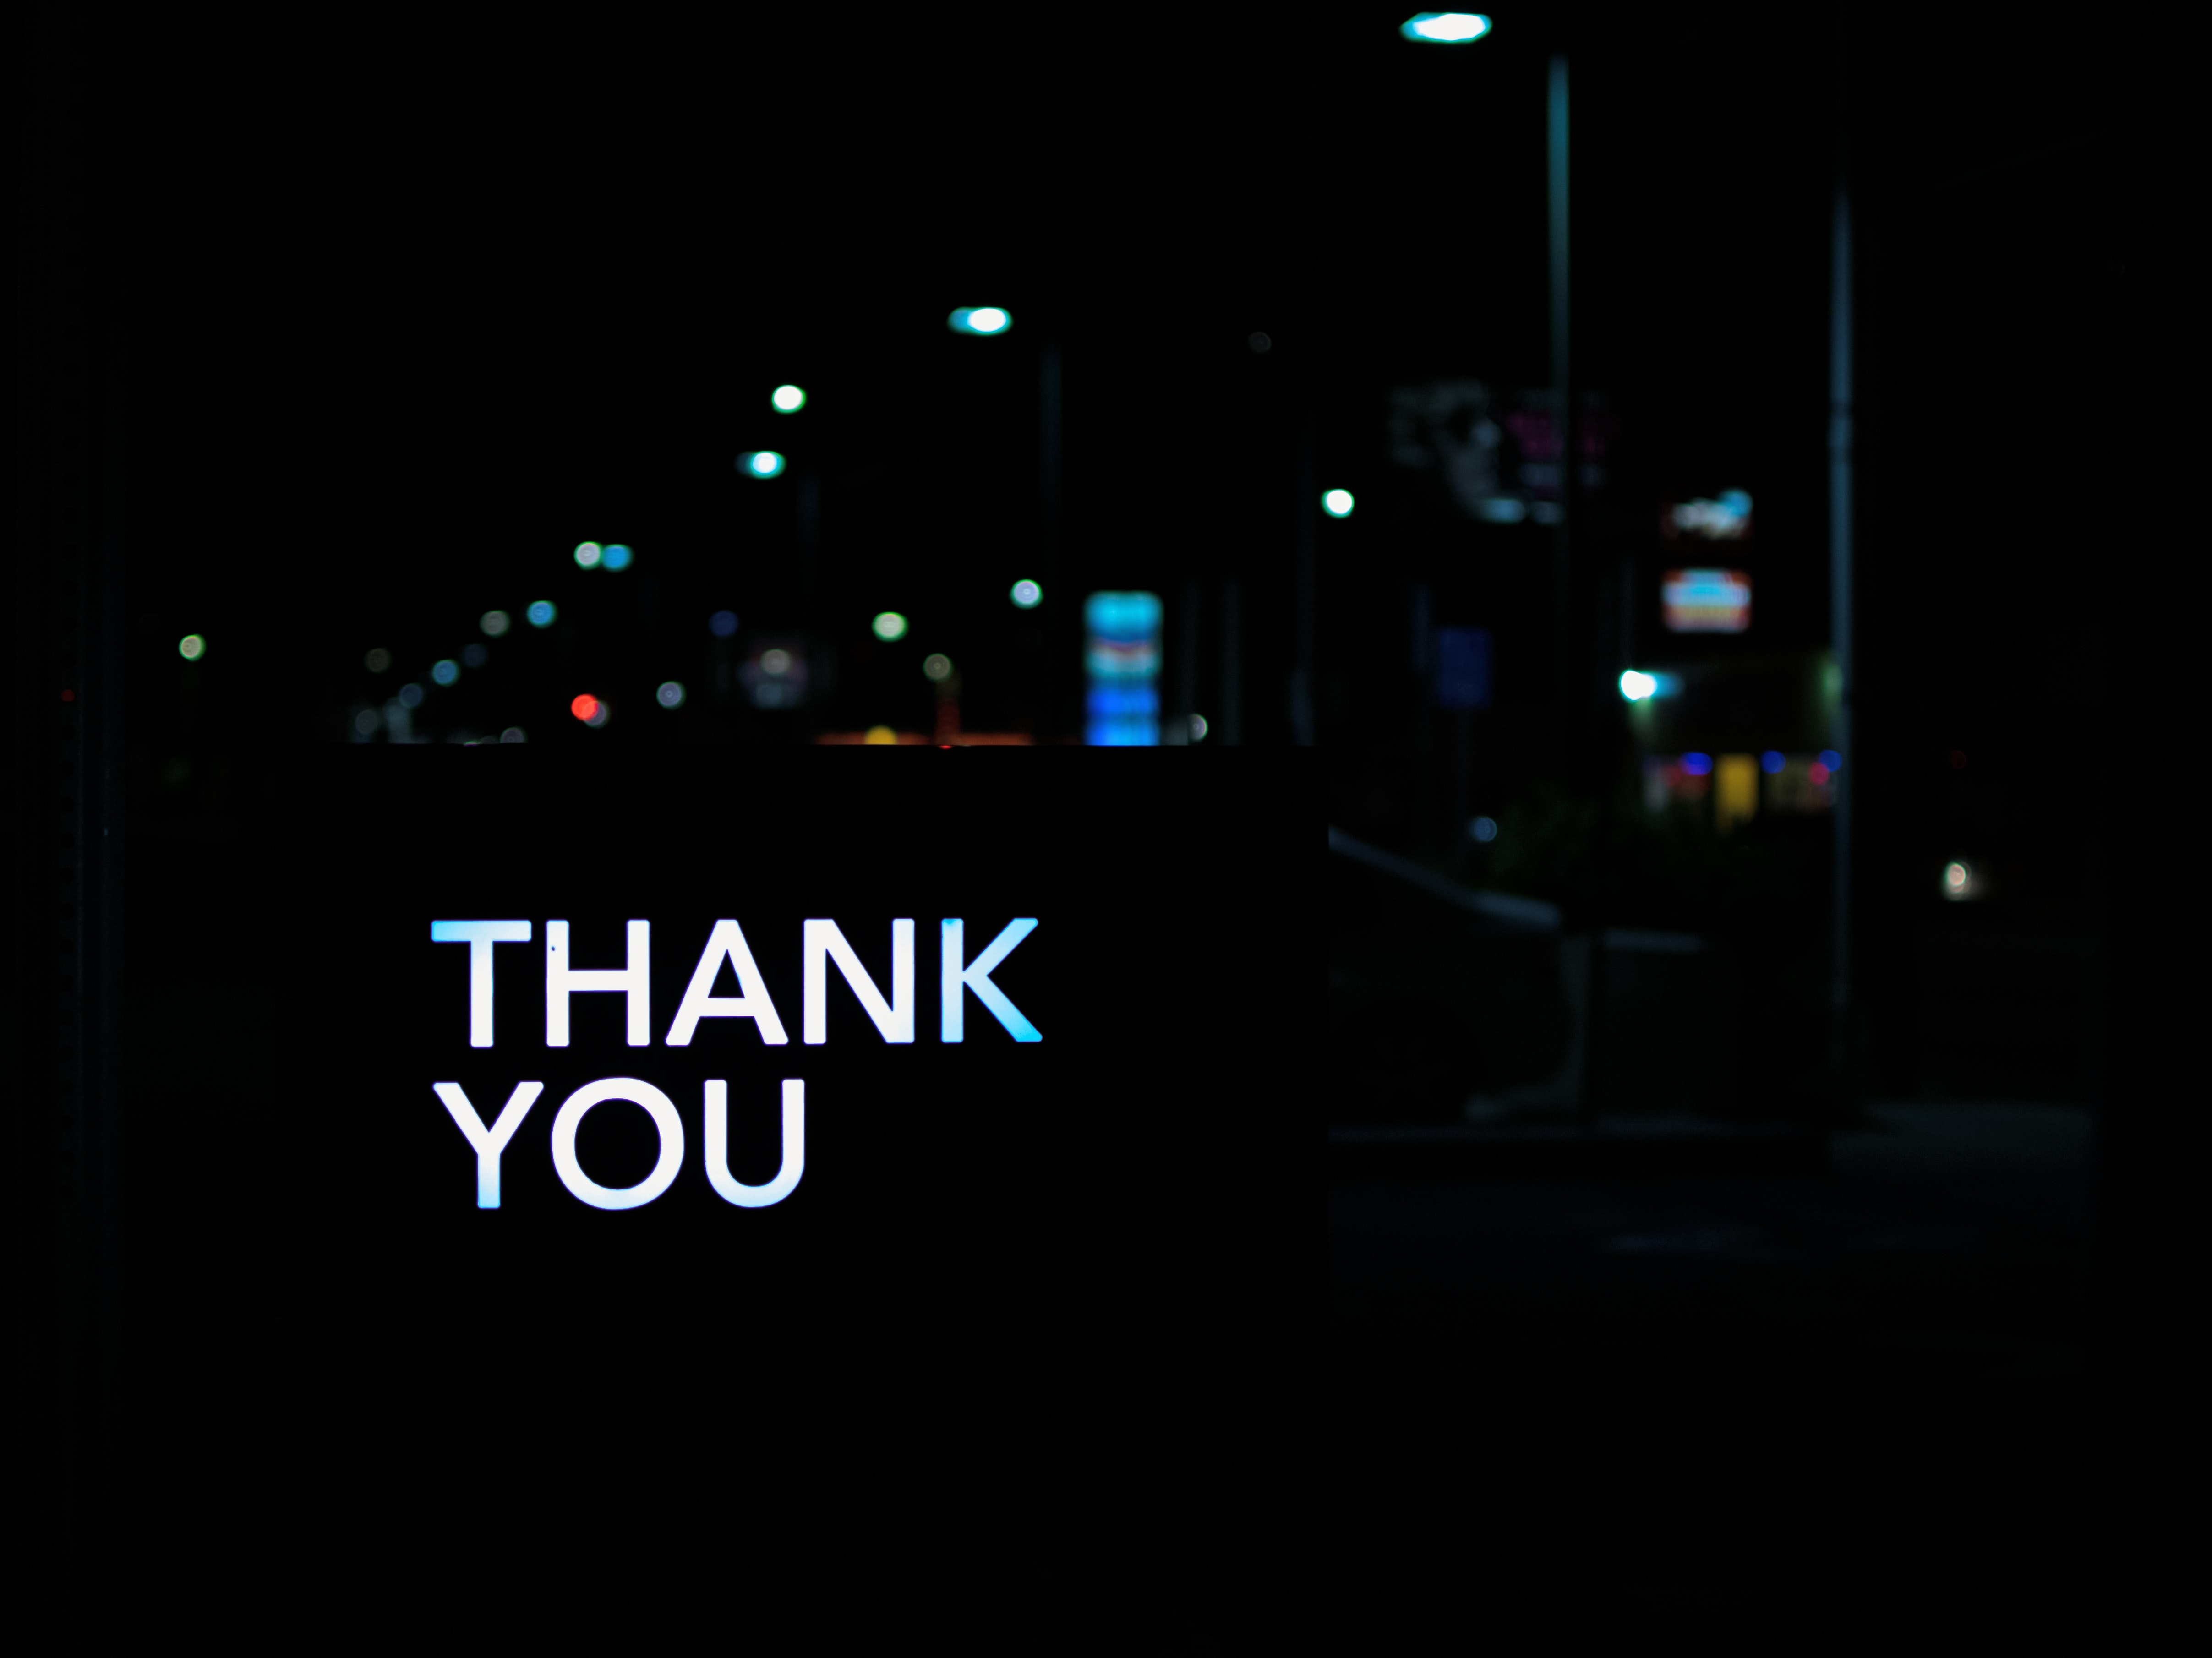
\includegraphics[width=1.2\paperwidth]{thanks.jpg}} 
\begin{frame}


$\,$\\[6cm] 
\end{frame}
}




%% %% %% %% Feedbackhinweisblock

% \begin{frame}
% \frametitle{Danke für Ihr Feedback!}

% \begin{columns}[c]

% \begin{column}{6cm}


% \begin{center}
%  \includegraphics[width=\textwidth]{smilie_balloons.jpg}
% \end{center}

% \end{column}

% \begin{column}{4cm}


% \begin{center}
% \includegraphics[width=\textwidth]{feedback_QR.png}
% \end{center}
% \end{column}


% \end{columns}
% \end{frame}


%% %% %% Bildnachweis
\begin{frame}
\frametitle{Bildnachweis}
\begin{tiny}

\begin{itemize}

\item
68-95-99.7 Regel.  By Melikamp - Own work, CC BY-SA 4.0, \url{https://commons.wikimedia.org/w/index.php?curid=65001875}

\item
Berge. Photo by \href{https://unsplash.com/@sepoys?utm_source=unsplash&utm_medium=referral&utm_content=creditCopyText}{Rohit Tandon} on \href{https://unsplash.com/s/photos/mountain?utm_source=unsplash&utm_medium=referral&utm_content=creditCopyText}{Unsplash}
  

\item
Boxer. Photo by \href{https://unsplash.com/@bayleejadegramling?utm_source=unsplash&utm_medium=referral&utm_content=creditCopyText}{Baylee Gramling} on \href{https://unsplash.com/s/photos/boxer?utm_source=unsplash&utm_medium=referral&utm_content=creditCopyText}{Unsplash}
  
  \item
Eigenschaften von Schwingungen. Meine eigene Arbeit, CC BY-SA 4.0 2022.

  
\item
Fortbewegung des Regenwurms. lilaandben. Der Regenwurm, 2022. \url{https://lilaundben.mediastart.de/de/gartenzwerg/der-regenwurm}

\item
Hörfläche. Von Hoerflaeche.svg: TehdogLukeTriton - Based on a SVG Drawing Datei:Hoerflaeche.svg.SVG drawing: Eigenes Werk (Originaltext: retraced as svg, copyright info taken from original), Gemeinfrei, \url{https://commons.wikimedia.org/w/index.php?curid=114265551}

\item

Maßband. Photo by \href{https://unsplash.com/@elisamichelet?utm_source=unsplash&utm_medium=referral&utm_content=creditCopyText}{Elisa Michelet} on \href{https://unsplash.com/s/photos/measurement?utm_source=unsplash&utm_medium=referral&utm_content=creditCopyText}{Unsplash}

  \item
  Phon und Dezibel. Der ursprünglich hochladende Benutzer war Skyhead in der Wikipedia auf Deutsch - Quelle für die zugrunde liegenden Daten:Vorlesungsscript "Akustik"; von J.Blauert, Ruhr-Universität Bochum, Gemeinfrei, \url{https://commons.wikimedia.org/w/index.php?curid=11918852}
  
  \item
Pirouette. Photo by \href{https://unsplash.com/@rodlong?utm_source=unsplash&utm_medium=referral&utm_content=creditCopyText}{Rod Long} on \href{https://unsplash.com/s/photos/figure-skater?utm_source=unsplash&utm_medium=referral&utm_content=creditCopyText}{Unsplash}  

\item
Sehr grobe Skizzen auf grünen Post-Its. Meine eigene Arbeit, CC-BY-SA 4.0, 2022.

\item
Seifenblasen. Photo by \href{https://unsplash.com/@kindandcurious?utm_source=unsplash&utm_medium=referral&utm_content=creditCopyText}{Kind and Curious} on \href{https://unsplash.com/s/photos/soap-bubble?utm_source=unsplash&utm_medium=referral&utm_content=creditCopyText}{Unsplash}  


\item
SI Einheiten. User:DePiep, CC BY-SA 3.0 \url{https://creativecommons.org/licenses/by-sa/3.0}, via Wikimedia Commons
% %%%%%%%%%%%

\item
Thank you. Photo by \href{https://unsplash.com/@peet818?utm_source=unsplash&utm_medium=referral&utm_content=creditCopyText}{Pete Pedroza} on \href{https://unsplash.com/s/photos/thank-you?utm_source=unsplash&utm_medium=referral&utm_content=creditCopyText}{Unsplash}
  

\item
  
Wanderweg mit Serpentinen. Von Nachtgiger - Image (picture) made by Nachtgiger, CC BY-SA 3.0, \url{https://commons.wikimedia.org/w/index.php?curid=6235458}. Version mit eingezeichneten Punkten und Wegen von mir, CC-BY-SA 3.0, 2022.


\item
Wippen. Photo by \href{https://unsplash.com/@candyflavor89?utm_source=unsplash&utm_medium=referral&utm_content=creditCopyText}{G T} on \href{https://unsplash.com/s/photos/seesaw?utm_source=unsplash&utm_medium=referral&utm_content=creditCopyText}{Unsplash}
  

\end{itemize}
\end{tiny}
\end{frame}






\end{document}

%%% Frequently used snippets

%% \begin{columns}[c]

%% \begin{column}{5cm}
%% \end{column}

%% \begin{column}{5cm}
%% \end{column}


%% \end{columns}




%% IMPP Frage

% \textbf{Frage} \\[0.2 cm]

% \begin{description}
% \item{A.}
% \item{B.}
% \item{C.}
% \item{D.}
% \item{E.}

% \end{description}